
%% bare_conf.tex
%% V1.3
%% 2007/01/11
%% by Michael Shell
%% See:
%% http://www.michaelshell.org/
%% for current contact information.
%%
%% This is a skeleton file demonstrating the use of IEEEtran.cls
%% (requires IEEEtran.cls version 1.7 or later) with an IEEE conference paper.
%%
%% Support sites:
%% http://www.michaelshell.org/tex/ieeetran/
%% http://www.ctan.org/tex-archive/macros/latex/contrib/IEEEtran/
%% and
%% http://www.ieee.org/

%%*************************************************************************
%% Legal Notice:
%% This code is offered as-is without any warranty either expressed or
%% implied; without even the implied warranty of MERCHANTABILITY or
%% FITNESS FOR A PARTICULAR PURPOSE!
%% User assumes all risk.
%% In no event shall IEEE or any contributor to this code be liable for
%% any damages or losses, including, but not limited to, incidental,
%% consequential, or any other damages, resulting from the use or misuse
%% of any information contained here.
%%
%% All comments are the opinions of their respective authors and are not
%% necessarily endorsed by the IEEE.
%%
%% This work is distributed under the LaTeX Project Public License (LPPL)
%% ( http://www.latex-project.org/ ) version 1.3, and may be freely used,
%% distributed and modified. A copy of the LPPL, version 1.3, is included
%% in the base LaTeX documentation of all distributions of LaTeX released
%% 2003/12/01 or later.
%% Retain all contribution notices and credits.
%% ** Modified files should be clearly indicated as such, including  **
%% ** renaming them and changing author support contact information. **
%%
%% File list of work: IEEEtran.cls, IEEEtran_HOWTO.pdf, bare_adv.tex,
%%                    bare_conf.tex, bare_jrnl.tex, bare_jrnl_compsoc.tex
%%*************************************************************************

% *** Authors should verify (and, if needed, correct) their LaTeX system  ***
% *** with the testflow diagnostic prior to trusting their LaTeX platform ***
% *** with production work. IEEE's font choices can trigger bugs that do  ***
% *** not appear when using other class files.                            ***
% The testflow support page is at:
% http://www.michaelshell.org/tex/testflow/



% Note that the a4paper option is mainly intended so that authors in
% countries using A4 can easily print to A4 and see how their papers will
% look in print - the typesetting of the document will not typically be
% affected with changes in paper size (but the bottom and side margins will).
% Use the testflow package mentioned above to verify correct handling of
% both paper sizes by the user's LaTeX system.
%
% Also note that the "draftcls" or "draftclsnofoot", not "draft", option
% should be used if it is desired that the figures are to be displayed in
% draft mode.
%
\documentclass[10pt, conference, compsocconf]{IEEEtran}
% Add the compsocconf option for Computer Society conferences.
%
% If IEEEtran.cls has not been installed into the LaTeX system files,
% manually specify the path to it like:
% \documentclass[conference]{../sty/IEEEtran}





% Some very useful LaTeX packages include:
% (uncomment the ones you want to load)


% *** MISC UTILITY PACKAGES ***
%
%\usepackage{ifpdf}
% Heiko Oberdiek's ifpdf.sty is very useful if you need conditional
% compilation based on whether the output is pdf or dvi.
% usage:
% \ifpdf
%   % pdf code
% \else
%   % dvi code
% \fi
% The latest version of ifpdf.sty can be obtained from:
% http://www.ctan.org/tex-archive/macros/latex/contrib/oberdiek/
% Also, note that IEEEtran.cls V1.7 and later provides a builtin
% \ifCLASSINFOpdf conditional that works the same way.
% When switching from latex to pdflatex and vice-versa, the compiler may
% have to be run twice to clear warning/error messages.






% *** CITATION PACKAGES ***
%
\usepackage{cite}
% cite.sty was written by Donald Arseneau
% V1.6 and later of IEEEtran pre-defines the format of the cite.sty package
% \cite{} output to follow that of IEEE. Loading the cite package will
% result in citation numbers being automatically sorted and properly
% "compressed/ranged". e.g., [1], [9], [2], [7], [5], [6] without using
% cite.sty will become [1], [2], [5]--[7], [9] using cite.sty. cite.sty's
% \cite will automatically add leading space, if needed. Use cite.sty's
% noadjust option (cite.sty V3.8 and later) if you want to turn this off.
% cite.sty is already installed on most LaTeX systems. Be sure and use
% version 4.0 (2003-05-27) and later if using hyperref.sty. cite.sty does
% not currently provide for hyperlinked citations.
% The latest version can be obtained at:
% http://www.ctan.org/tex-archive/macros/latex/contrib/cite/
% The documentation is contained in the cite.sty file itself.






% *** GRAPHICS RELATED PACKAGES ***
%
\usepackage{graphicx}
\ifCLASSINFOpdf
  % \usepackage[pdftex]{graphicx}
  % declare the path(s) where your graphic files are
  % \graphicspath{{../pdf/}{../jpeg/}}
  % and their extensions so you won't have to specify these with
  % every instance of \includegraphics
  % \DeclareGraphicsExtensions{.pdf,.jpeg,.png}
\else
  % or other class option (dvipsone, dvipdf, if not using dvips). graphicx
  % will default to the driver specified in the system graphics.cfg if no
  % driver is specified.
   \usepackage[dvips]{graphicx}
  % declare the path(s) where your graphic files are
  % \graphicspath{{../eps/}}
  % and their extensions so you won't have to specify these with
  % every instance of \includegraphics
  % \DeclareGraphicsExtensions{.eps}
\fi
% graphicx was written by David Carlisle and Sebastian Rahtz. It is
% required if you want graphics, photos, etc. graphicx.sty is already
% installed on most LaTeX systems. The latest version and documentation can
% be obtained at:
% http://www.ctan.org/tex-archive/macros/latex/required/graphics/
% Another good source of documentation is "Using Imported Graphics in
% LaTeX2e" by Keith Reckdahl which can be found as epslatex.ps or
% epslatex.pdf at: http://www.ctan.org/tex-archive/info/
%
% latex, and pdflatex in dvi mode, support graphics in encapsulated
% postscript (.eps) format. pdflatex in pdf mode supports graphics
% in .pdf, .jpeg, .png and .mps (metapost) formats. Users should ensure
% that all non-photo figures use a vector format (.eps, .pdf, .mps) and
% not a bitmapped formats (.jpeg, .png). IEEE frowns on bitmapped formats
% which can result in "jaggedy"/blurry rendering of lines and letters as
% well as large increases in file sizes.
%
% You can find documentation about the pdfTeX application at:
% http://www.tug.org/applications/pdftex





% *** MATH PACKAGES ***
%
\usepackage[cmex10]{amsmath}
% A popular package from the American Mathematical Society that provides
% many useful and powerful commands for dealing with mathematics. If using
% it, be sure to load this package with the cmex10 option to ensure that
% only type 1 fonts will utilized at all point sizes. Without this option,
% it is possible that some math symbols, particularly those within
% footnotes, will be rendered in bitmap form which will result in a
% document that can not be IEEE Xplore compliant!
%
% Also, note that the amsmath package sets \interdisplaylinepenalty to 10000
% thus preventing page breaks from occurring within multiline equations. Use:
%\interdisplaylinepenalty=2500
% after loading amsmath to restore such page breaks as IEEEtran.cls normally
% does. amsmath.sty is already installed on most LaTeX systems. The latest
% version and documentation can be obtained at:
% http://www.ctan.org/tex-archive/macros/latex/required/amslatex/math/





% *** SPECIALIZED LIST PACKAGES ***
%
\usepackage{algorithmic}
\usepackage{algorithm}
% algorithmic.sty was written by Peter Williams and Rogerio Brito.
% This package provides an algorithmic environment fo describing algorithms.
% You can use the algorithmic environment in-text or within a figure
% environment to provide for a floating algorithm. Do NOT use the algorithm
% floating environment provided by algorithm.sty (by the same authors) or
% algorithm2e.sty (by Christophe Fiorio) as IEEE does not use dedicated
% algorithm float types and packages that provide these will not provide
% correct IEEE style captions. The latest version and documentation of
% algorithmic.sty can be obtained at:
% http://www.ctan.org/tex-archive/macros/latex/contrib/algorithms/
% There is also a support site at:
% http://algorithms.berlios.de/index.html
% Also of interest may be the (relatively newer and more customizable)
% algorithmicx.sty package by Szasz Janos:
% http://www.ctan.org/tex-archive/macros/latex/contrib/algorithmicx/




% *** ALIGNMENT PACKAGES ***
%
%\usepackage{array}
% Frank Mittelbach's and David Carlisle's array.sty patches and improves
% the standard LaTeX2e array and tabular environments to provide better
% appearance and additional user controls. As the default LaTeX2e table
% generation code is lacking to the point of almost being broken with
% respect to the quality of the end results, all users are strongly
% advised to use an enhanced (at the very least that provided by array.sty)
% set of table tools. array.sty is already installed on most systems. The
% latest version and documentation can be obtained at:
% http://www.ctan.org/tex-archive/macros/latex/required/tools/


%\usepackage{mdwmath}
%\usepackage{mdwtab}
% Also highly recommended is Mark Wooding's extremely powerful MDW tools,
% especially mdwmath.sty and mdwtab.sty which are used to format equations
% and tables, respectively. The MDWtools set is already installed on most
% LaTeX systems. The lastest version and documentation is available at:
% http://www.ctan.org/tex-archive/macros/latex/contrib/mdwtools/


% IEEEtran contains the IEEEeqnarray family of commands that can be used to
% generate multiline equations as well as matrices, tables, etc., of high
% quality.


%\usepackage{eqparbox}
% Also of notable interest is Scott Pakin's eqparbox package for creating
% (automatically sized) equal width boxes - aka "natural width parboxes".
% Available at:
% http://www.ctan.org/tex-archive/macros/latex/contrib/eqparbox/





% *** SUBFIGURE PACKAGES ***
\usepackage[tight,footnotesize]{subfigure}
% subfigure.sty was written by Steven Douglas Cochran. This package makes it
% easy to put subfigures in your figures. e.g., "Figure 1a and 1b". For IEEE
% work, it is a good idea to load it with the tight package option to reduce
% the amount of white space around the subfigures. subfigure.sty is already
% installed on most LaTeX systems. The latest version and documentation can
% be obtained at:
% http://www.ctan.org/tex-archive/obsolete/macros/latex/contrib/subfigure/
% subfigure.sty has been superceeded by subfig.sty.



%\usepackage[caption=false]{caption}
%\usepackage[font=footnotesize]{subfig}
\usepackage{caption}
\usepackage{subfigure}
% subfig.sty, also written by Steven Douglas Cochran, is the modern
% replacement for subfigure.sty. However, subfig.sty requires and
% automatically loads Axel Sommerfeldt's caption.sty which will override
% IEEEtran.cls handling of captions and this will result in nonIEEE style
% figure/table captions. To prevent this problem, be sure and preload
% caption.sty with its "caption=false" package option. This is will preserve
% IEEEtran.cls handing of captions. Version 1.3 (2005/06/28) and later
% (recommended due to many improvements over 1.2) of subfig.sty supports
% the caption=false option directly:
%\usepackage[caption=false,font=footnotesize]{subfig}
%
% The latest version and documentation can be obtained at:
% http://www.ctan.org/tex-archive/macros/latex/contrib/subfig/
% The latest version and documentation of caption.sty can be obtained at:
% http://www.ctan.org/tex-archive/macros/latex/contrib/caption/




% *** FLOAT PACKAGES ***
%
%\usepackage{fixltx2e}
% fixltx2e, the successor to the earlier fix2col.sty, was written by
% Frank Mittelbach and David Carlisle. This package corrects a few problems
% in the LaTeX2e kernel, the most notable of which is that in current
% LaTeX2e releases, the ordering of single and double column floats is not
% guaranteed to be preserved. Thus, an unpatched LaTeX2e can allow a
% single column figure to be placed prior to an earlier double column
% figure. The latest version and documentation can be found at:
% http://www.ctan.org/tex-archive/macros/latex/base/



%\usepackage{stfloats}
\usepackage{float}
% stfloats.sty was written by Sigitas Tolusis. This package gives LaTeX2e
% the ability to do double column floats at the bottom of the page as well
% as the top. (e.g., "\begin{figure*}[!b]" is not normally possible in
% LaTeX2e). It also provides a command:
%\fnbelowfloat
% to enable the placement of footnotes below bottom floats (the standard
% LaTeX2e kernel puts them above bottom floats). This is an invasive package
% which rewrites many portions of the LaTeX2e float routines. It may not work
% with other packages that modify the LaTeX2e float routines. The latest
% version and documentation can be obtained at:
% http://www.ctan.org/tex-archive/macros/latex/contrib/sttools/
% Documentation is contained in the stfloats.sty comments as well as in the
% presfull.pdf file. Do not use the stfloats baselinefloat ability as IEEE
% does not allow \baselineskip to stretch. Authors submitting work to the
% IEEE should note that IEEE rarely uses double column equations and
% that authors should try to avoid such use. Do not be tempted to use the
% cuted.sty or midfloat.sty packages (also by Sigitas Tolusis) as IEEE does
% not format its papers in such ways.





% *** PDF, URL AND HYPERLINK PACKAGES ***
%
%\usepackage{url}
% url.sty was written by Donald Arseneau. It provides better support for
% handling and breaking URLs. url.sty is already installed on most LaTeX
% systems. The latest version can be obtained at:
% http://www.ctan.org/tex-archive/macros/latex/contrib/misc/
% Read the url.sty source comments for usage information. Basically,
% \url{my_url_here}.





% *** Do not adjust lengths that control margins, column widths, etc. ***
% *** Do not use packages that alter fonts (such as pslatex).         ***
% There should be no need to do such things with IEEEtran.cls V1.6 and later.
% (Unless specifically asked to do so by the journal or conference you plan
% to submit to, of course. )


% correct bad hyphenation here
\hyphenation{op-tical net-works semi-conduc-tor}


\begin{document}
%
% paper title
% can use linebreaks \\ within to get better formatting as desired
\title{A Feature Preserved Mesh Subdivision Framework for Biomedical Mesh}


% author names and affiliations
% use a multiple column layout for up to two different
% affiliations

%\author{
%\IEEEauthorblockN{Jing Yang, Yongyi Gong, Hefeng Wu}
%\IEEEauthorblockA{School of Information Science and Technology\\
%Guangdong University of Foreign Studies\\
%Guangzhou, China\\
%jingyang\_carl@qq.com}
%\and
%\IEEEauthorblockN{Qi Li}
%\IEEEauthorblockA{Department of Computer Science\\
%Western Kentucky University\\
%Bowling Green, KY, USA\\
%}
%}
\author{\IEEEauthorblockN{Jing Yang$^{\dag}$, Yongyi Gong$^{\dag}$, Hefeng Wu$^{\dag}$, and Qi Li$^{\ddag}$}
\IEEEauthorblockA{$^{\dag}$School of Information Science and Technology, Guangdong University of Foreign Studies, China}
\IEEEauthorblockA{$^{\ddag}$Department of Computer Science, Western Kentucky University, Bowling Green, KY, USA}
\textit{jingyang.carl.china@gmail.com, gongyongyi@gdufs.edu.cn, wuhefeng@gmail.com, qi.li@wku.edu}
}

% conference papers do not typically use \thanks and this command
% is locked out in conference mode. If really needed, such as for
% the acknowledgment of grants, issue a \IEEEoverridecommandlockouts
% after \documentclass

% for over three affiliations, or if they all won't fit within the width
% of the page, use this alternative format:
%
%\author{\IEEEauthorblockN{Michael Shell\IEEEauthorrefmark{1},
%Homer Simpson\IEEEauthorrefmark{2},
%James Kirk\IEEEauthorrefmark{3},
%Montgomery Scott\IEEEauthorrefmark{3} and
%Eldon Tyrell\IEEEauthorrefmark{4}}
%\IEEEauthorblockA{\IEEEauthorrefmark{1}School of Electrical and Computer Engineering\\
%Georgia Institute of Technology,
%Atlanta, Georgia 30332--0250\\ Email: see http://www.michaelshell.org/contact.html}
%\IEEEauthorblockA{\IEEEauthorrefmark{2}Twentieth Century Fox, Springfield, USA\\
%Email: homer@thesimpsons.com}
%\IEEEauthorblockA{\IEEEauthorrefmark{3}Starfleet Academy, San Francisco, California 96678-2391\\
%Telephone: (800) 555--1212, Fax: (888) 555--1212}
%\IEEEauthorblockA{\IEEEauthorrefmark{4}Tyrell Inc., 123 Replicant Street, Los Angeles, California 90210--4321}}




% use for special paper notices
%\IEEEspecialpapernotice{(Invited Paper)}




% make the title area
\maketitle


\begin{abstract}
As biomedical data in 3D space collected increasingly, there is a pressing need for efficient and accurate applications in the field of bioinformation analysis. For biomedical purpose, mesh subdivision techniques are commonly used to generate adaptive multi-resolution meshes for fast or accurate algorithms. However, current smoothing methods for each subdivision algorithm will moderate edge and vertex features from the original mesh. In this paper, we propose a feature preserved mesh subdivision framework, which generates a visually sensitive and a more precise result compared with commonly used subdivision methods, to preserve edge and vertex geometrical features of biomedical data.

\end{abstract}

\begin{IEEEkeywords}
mesh subdivision, keypoints, feature preserved, biomedical mesh

\end{IEEEkeywords}


% For peer review papers, you can put extra information on the cover
% page as needed:
% \ifCLASSOPTIONpeerreview
% \begin{center} \bfseries EDICS Category: 3-BBND \end{center}
% \fi
%
% For peerreview papers, this IEEEtran command inserts a page break and
% creates the second title. It will be ignored for other modes.
\IEEEpeerreviewmaketitle

%%%%%%%%%%%%%%%%%%%%%%%%%%%%%%%%%%%%%%%%%%%%%%%%%%%%%%%%%%%%%%%%%%%%%%%%%%%%%%%%%%%%%%%%%%%%%%%%%%%%%%%%
%%%%%%%%%%%%%%%%%%%%%%%%%%%%%%%%%%%%%%%%%%%%%%%%%%%%%%%%%%%%%%%%%%%%%%%%%%%%%%%%%%%%%%%%%%%%%%%%%%%%%%%%

\section{Introduction}
% no \IEEEPARstart

%%Figure_EFPMS
\begin{figure*}[htb]
  \centering
%  \captionsetup{justification=centering,margin=1cm}

  \subfigure[Original]{
      \begin{minipage}[h]{0.2\linewidth}
        \centering
        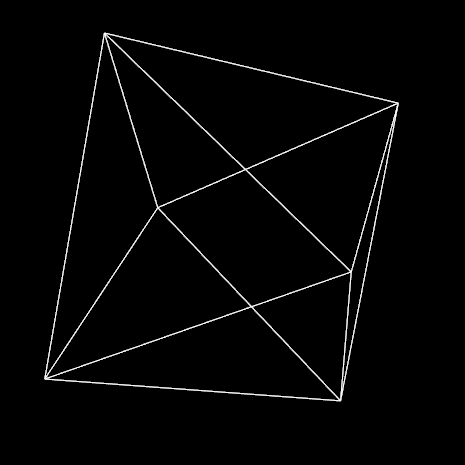
\includegraphics[width=\textwidth]{./Figure/octahedron/original-.png}\\
        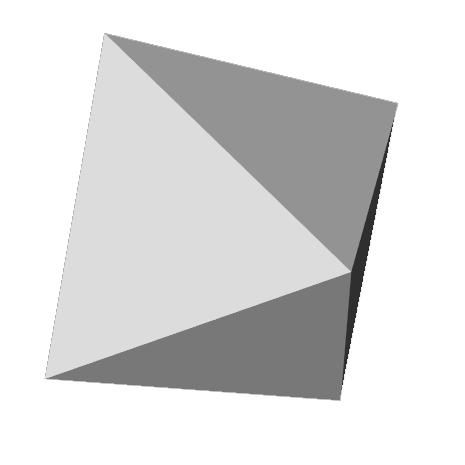
\includegraphics[width=\textwidth]{./Figure/octahedron/original.png}\\
      \end{minipage}
  }%
  \hskip -2ex
  \subfigure[Butterfly]{
      \begin{minipage}[h]{0.2\linewidth}
        \centering
        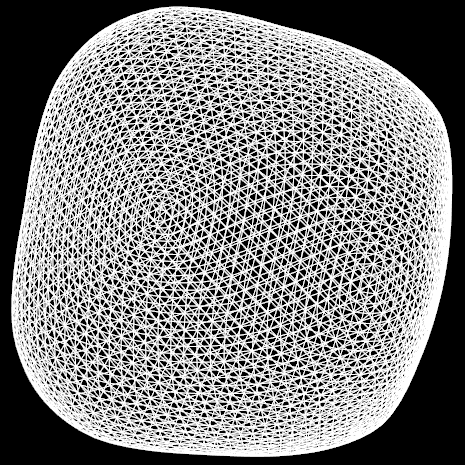
\includegraphics[width=\textwidth]{./Figure/octahedron/butterfly-.png}\\
        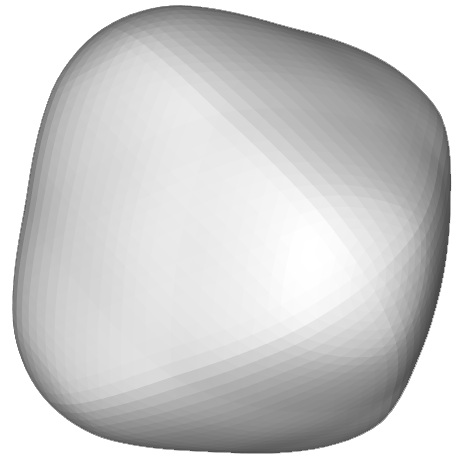
\includegraphics[width=\textwidth]{./Figure/octahedron/butterfly.png}\\
      \end{minipage}
  }%
  \hskip -2ex
  \subfigure[Loop]{
      \begin{minipage}[h]{0.2\linewidth}
        \centering
        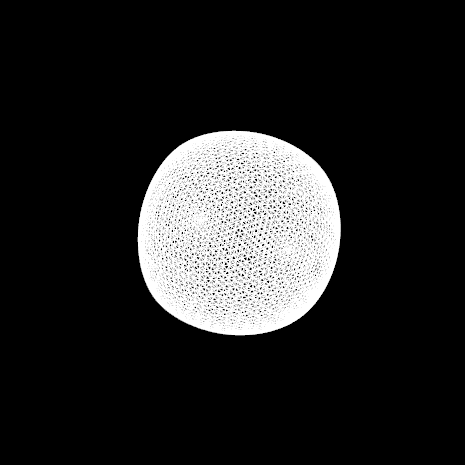
\includegraphics[width=\textwidth]{./Figure/octahedron/loop-.png}\\
        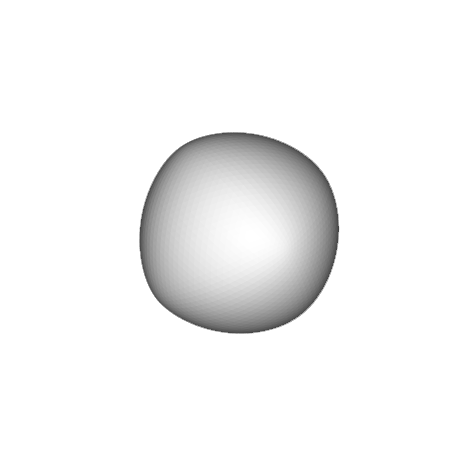
\includegraphics[width=\textwidth]{./Figure/octahedron/loop.png}\\
      \end{minipage}
  }%
  \hskip -2ex
  \subfigure[Catmull]{
      \begin{minipage}[h]{0.2\linewidth}
        \centering
        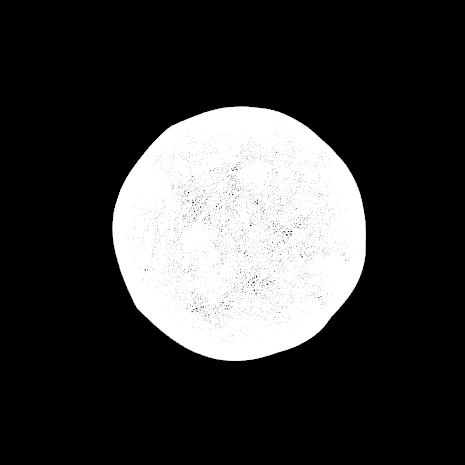
\includegraphics[width=\textwidth]{./Figure/octahedron/catmull-.png}\\
        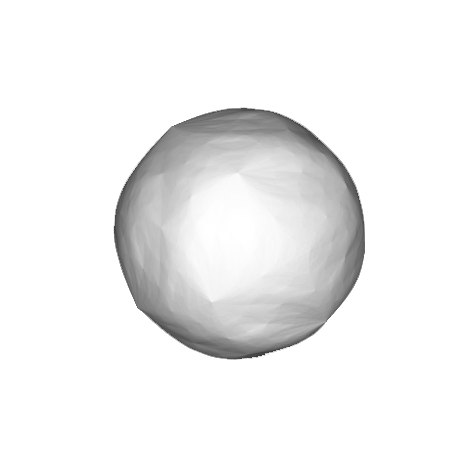
\includegraphics[width=\textwidth]{./Figure/octahedron/catmull.png}\\
      \end{minipage}
  }%
  \hskip -2ex
  \subfigure[EFPMS]{
      \begin{minipage}[h]{0.2\linewidth}
        \centering
        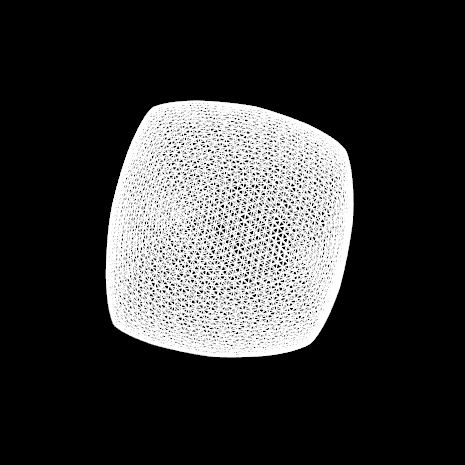
\includegraphics[width=\textwidth]{./Figure/octahedron/weight2-.png}\\
        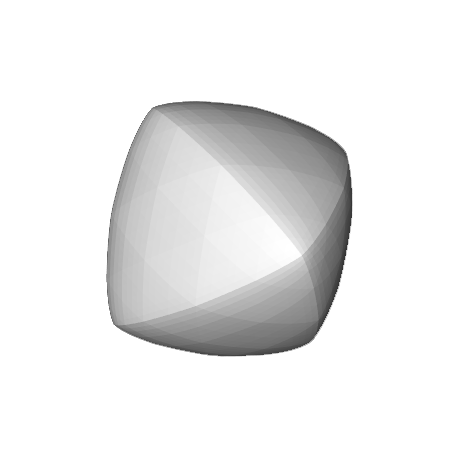
\includegraphics[width=\textwidth]{./Figure/octahedron/weight2.png}\\
      \end{minipage}
  }

  \caption{Demonstration of different subdivision methods. a) Original Mesh. b) Butterfly Subdivision. c) Loop Subdivision. d) Catmull Subdivision. e) Edge Feature Preserved Mesh Subdivision (implementation of our framework's core module). All subdivision algorithms have been applied five iterations on original mesh.}\label{Figure_EFPMS}
\end{figure*}

In recent years, 3D computer graphical technology works diffusely as biomedical assistants, including utilizations of three dimensional CT (3D CT) reconstructions \cite{Choi2016Acceleration,koopman2016small,Muthusami2017CT,Mccann2016Fast}, presentations of skeletons and tissues \cite{Tao1999Application}, comparisons of genome \cite{Lein2007Genome,Bonev2016Organization,Tjong2016Population,Caspermeyer2017Principles}, etc., due to its visual obviousness. The technique is widely used for presenting facial bones and their connections, confirmation of borderline or size of diseased tissues and their relation to the adjacent tissues. With the aid of bio-images and bio-models, diagnosis and operations on clinical medicine achieves a much higher precision. Moreover, substantial effort has been made around world to determine spatial expression patterns of genes in mammalian genome using experimental techniques such as in situ hybridization (ISH) \cite{Carson2002A}. Performing ISH on multiple subjects yields expression images of various genes over the common anatomical structure and comparing these images reveals the spatial relations between genes, which are often key to understanding their functional relations \cite{Ju2003A,Schaefer2004Smooth}.

The pros of using computer graphics including 3D spatial and triangular meshes \cite{B2014Interactive,Guskov2014Non,Zhang2015A} to expose the nicety of bioinformation has created an ever-titanic amount of spatial data (in the form of 2D medical images and 3D bio-models) which requires efficient and accurate processing and analysis consequently. The anatomical differentiations among these biomedical models aggravate the computational challenges involved in visual and medical comparison among data collected from different modes \cite{Tao2010Subdivision}.

Restrained by the calculation performance of physical devices, medical detailed expression and accuracy of biomedical data
%, in which the rudimentary expression are 3D meshes (triangular form, quad form, combined form),
is unfavorably circumstanced. Solutions emerge as medical processing requires, one of which is using meshes without redundant vertices and faces. The contradiction of biomedical precision and data optimization will become serious as models shrink. Hence, feature-based mesh subdivision present state-of-the-art results\cite{Tao2010Subdivision}.

Using feature-based subdivision to suitably amplify medical precision and organize spatial data into multi-resolution versions, visual comparison and diagnosis will have a higher performance\cite{Tao2010Subdivision}. Meanwhile, the multi-resolution structure of a subdivision mesh further gives rise to fast algorithms for processing and accurate comparison for tiny bio-divergence.

Commonly used mesh subdivision methods including Butterfly method \cite{Zorin1996Interpolating}, Loop subdivision \cite{Loop1987Smooth}, and Catmull-Clark subdivision \cite{Catmull1978Recursively}, whose experimental results are illustrated in Fig. \ref{Figure_EFPMS}. Moreover, Xie et al. \cite{Xie2015Drape} provided a solid-shell element based triangular subdivision to avoid interpenetration. Liu \cite{Liu2014An} introduced a dense reconstruction algorithm for mesh subdivision. Amresh et al. \cite{Amresh2002Adaptive} developed a subdivision scheme derived from Loop scheme and using watershed segmentation. Rose et al. \cite{Rose2001On} proposed an adaptive process that stores the next splitting vertex and temporary triangle based on Modified Butterfly scheme. Kobbelt \cite{Kobbelt2000} developed refinement for both his Kobbelt scheme and newly introduced $\sqrt{3}$ subdivision. Seeger and Kai \cite{Seeger2001A} introduced a subdivision scheme based on Butterfly Scheme using quark. In their method, subdivision is controlled by the faces of the original mesh and mesh features that are not suitably preserved.

In this paper, we propose a feature preserved mesh subdivision framework to maintain geometrical features, including edges and imbalanced vertices, of original biomedical meshes while giving out a more adaptive mesh derivative. Our contributions include: a) imbalanced keypoint detection for point feature preservation, b) edge feature preserved mesh subdivision for edge feature preservation, and c) model-dependent wavelike noise elimination for result optimization. Subdivision results will be compared after the same number of iterations and results show the promise of our method on feature maintained mesh subdivisions.

%The rest of the paper is organized as follows: In Section \ref{Section:Fundamental Subalgorithms}, we present an imbalanced keypoint detection method to locate features on meshes, and provide our basic idea of Edge Feature Preserved Mesh Subdivision with its improved version to efface model-dependent noise wave on the mesh. Then in Section \ref{Section:Keypoint based Feature Preserved Mesh Subdivision Scheme}, we combine keypoint detection method with our edge subdivision algorithm to establish Feature Preserved Mesh Subdivision Framework. Moreover, experimental comparison and conclusion will be arranged in Section \ref{Section:Experiment} and Section \ref{Section:Conclusion}, respectively.

%%%%%%%%%%%%%%%%%%%%%%%%%%%%%%%%%%%%%%%%%%%%%%%%%%%%%%%%%%%%%%%%%%%%%%%%%%%%%%%%%%%%%%%%%%%%%%%%%%%%%%%%
%%%%%%%%%%%%%%%%%%%%%%%%%%%%%%%%%%%%%%%%%%%%%%%%%%%%%%%%%%%%%%%%%%%%%%%%%%%%%%%%%%%%%%%%%%%%%%%%%%%%%%%%

\section{Coupling Modules of Subdivision Framework: Fundamental Subalgorithms}\label{Section:Fundamental Subalgorithms}
In this section, we will give an overview of algorithm modules within the proposed framework where Imbalanced Keypoint Detection focuses on vertex features while Edge Feature Preserved Mesh Subdivision (EFPMS) underscores edge features. A brief introduction on imbalanced-vertex based feature detection will first be presented and then our algorithm kernel, EFPMS, are provided, while a corresponding optimization solution is proposed afterward to eliminate model-dependent wavelike noise generated from that. Moreover, the kernel module follows subdivision scheme composed of linear triangular face subdivision and vertex smoothing.

%%%%%%%%%%%%%%%%%%%%%%%%%%%%%%%%%%%%%%%%%%%%%%%%%%%%%%%%%%%%%%%%%%%%%%%%%%%%%%%%%%%%%%%%%%%%%%%%%%%%%%%%

\subsection{Imbalanced Keypoint Detection}
We first propose a geometric feature-based vertex operator, which is a three-dimensional implementation of keypoints detection, to pick up imbalanced keypoints. We extend Li's  previous work \cite{Li2008Interest} on imbalanced keypoints detection to triangular meshes.

\begin{figure}[!tb]
  \centering
%  \captionsetup{justification=centering,margin=0cm}
  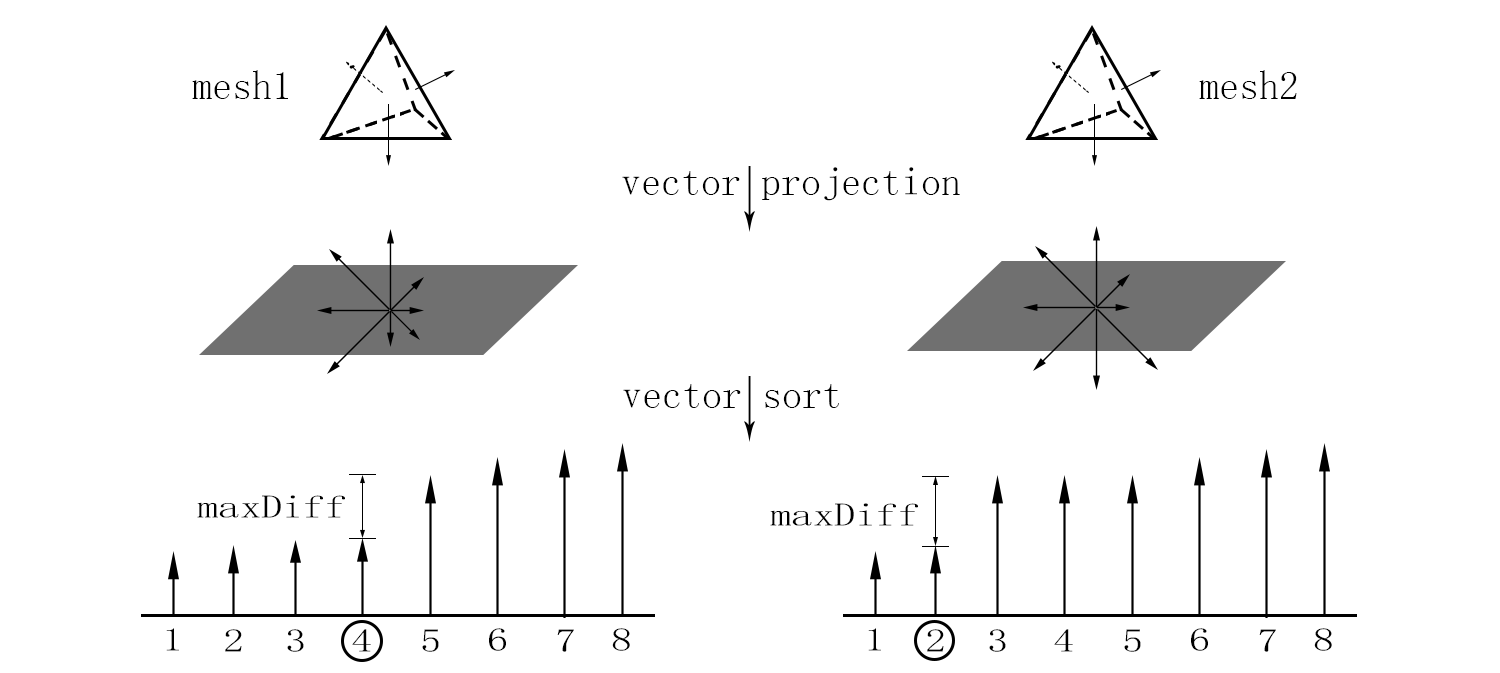
\includegraphics[width=\linewidth]{./Figure/ImbalancedKeypointsDetection.png}
  \caption{Illustration of imbalance selection. After projecting face normals around vertex on its tangent plane, projected normals (suppose 8 directions) are sorted in terms of their magnitudes. Left: balanced edge point, where index of maximum difference is 4. Right: imbalanced edge point, where that is 2.}\label{Figure_Imbalanced_Keypoint_Selection}
\end{figure}

The basic idea of vertex operator is using projections to transform 3D geometric features to two-dimensional space. Let $M(V,F,N_F)$ be a triangular mesh where $V$ is the set of vertices, $F$ is the set of faces, and $N_F$ represents the set of face normals. Suppose a projection $P_T$ will project any vector onto the plane $T$, 3D geometric mesh features will be transformed to two dimensions when $T$ is the tangent plane of the given mesh vertex in vertex set $V$. Face normals $N_F$ will then be transformed into its projected vector set $N_F\prime$. Finally, we settle all normalized vectors in $N_F\prime$ to a polar coordinate system and calculate the set of cross angles between each vector side by side, denote as $A_F$.

Imbalanced point selection in 2D images aims to minimize the occurrences of edge points\cite{Li2008Interest} as illustrated in Fig. \ref{Figure_Imbalanced_Keypoint_Selection}. Denote $I$ a grayscale image, $p$ a local point, $\theta_i=\frac{(i-1)2\pi}{N}$, and $l_i=(\cos\theta_i ,\sin\theta_i)$ for $i=1,2,...,N$. Denote $\frac{\partial{I}}{\partial{l_i}}(p)$ a directional derivative of $p$ along $l_i$ direction. We cluster $\{\frac{\partial{I}}{\partial{l_i}}(p)\}^{N}_{i=1}$ into two classes in terms of their magnitudes $|\frac{\partial{I}}{\partial{l_i}}(p)|$. If two clusters have the same size, the image point $p$ is balanced.

The sorting method proposed in Li's method is to classify $\{\frac{\partial{I}}{\partial{l_i}}(p)\}^{N}_{i=1}$, which can be generalized to extract 3D imbalanced vertices with proposed operator. Let $maxDiff$ be the max difference and $D$ be the index of maximum difference:

\begin{equation}\label{Equation_MaxDiff}
  maxDiff=\max_j(\alpha_{j+1}-\alpha_j)
\end{equation}

\begin{equation}\label{Equation_D}
  D=\mathop{\arg\min}_{j}(\alpha_{j+1}-\alpha_j)
\end{equation}
where $\alpha$ represents value in $A_F$, and $1\leq{j}\leq{N-1}$. Given a threshold on homogeneity $\varepsilon$, the imbalanced vertex can be defined under the condition that $maxDiff<\varepsilon$:

\begin{equation}\label{Equation_IMB}
  IMB(v_i)=
    \begin{cases}
    1& \text{$D_i<\frac{N}{2}$} \\
    0& \text{else}
    \end{cases}
\end{equation}

One of the implementation results is presented in Fig. \ref{Figure_Keypoints} where imbalanced keypoints delineate vertex features.

\begin{figure}[htbp]
  \centering
%  \captionsetup{justification=centering,margin=0.2cm}

      \begin{minipage}[h]{0.48\linewidth}
        \centering
        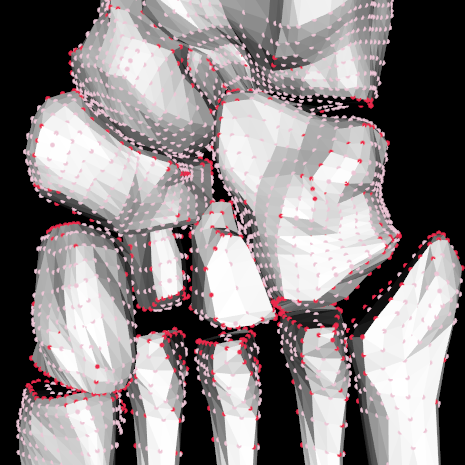
\includegraphics[width=\textwidth]{./Figure/keypoint/front.png}\\
      \end{minipage}%
      \begin{minipage}[h]{0.48\linewidth}
        \centering
        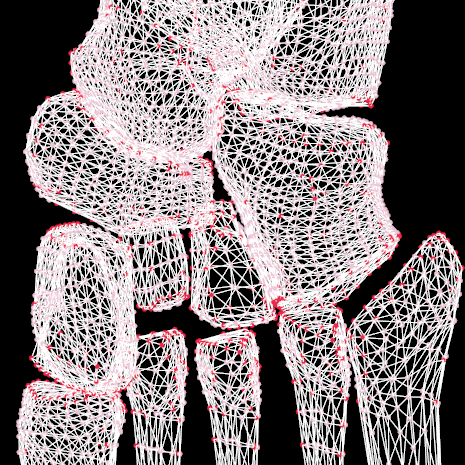
\includegraphics[width=\textwidth]{./Figure/keypoint/front-.png}\\
      \end{minipage}
  \caption{Imbalanced keypoints on footbone mesh with white points representing normal points and red for imbalanced points. Left: model view. Right: mesh view.}\label{Figure_Keypoints}
\end{figure}

%%%%%%%%%%%%%%%%%%%%%%%%%%%%%%%%%%%%%%%%%%%%%%%%%%%%%%%%%%%%%%%%%%%%%%%%%%%%%%%%%%%%%%%%%%%%%%%%%%%%%%%%

\subsection{Edge Feature Preserved Mesh Subdivision}
Loops method \cite{Loop1987Smooth} can be expressed as linear subdivision and an averaging scheme to approximate a spherical surface, which will efface edge and vertex features. The phenomenon is common when applying Catmull method and Butterfly method. When the mesh is rigid, these iterations will fail to preserve the original geometrical features as illustrated in Fig. \ref{Figure_EFPMS}. To moderate the feature friction after subdivision and highlight original edge and vertex features, we provide an Edge Feature Preserved Mesh Subdivision (EFPMS) method to generate feature adaptive results, where the pseudocode is arranged in Algorithm \ref{Algorithm_EFPMS}.

\begin{figure}[htbp]
  \centering
%  \captionsetup{justification=centering,margin=1cm}
  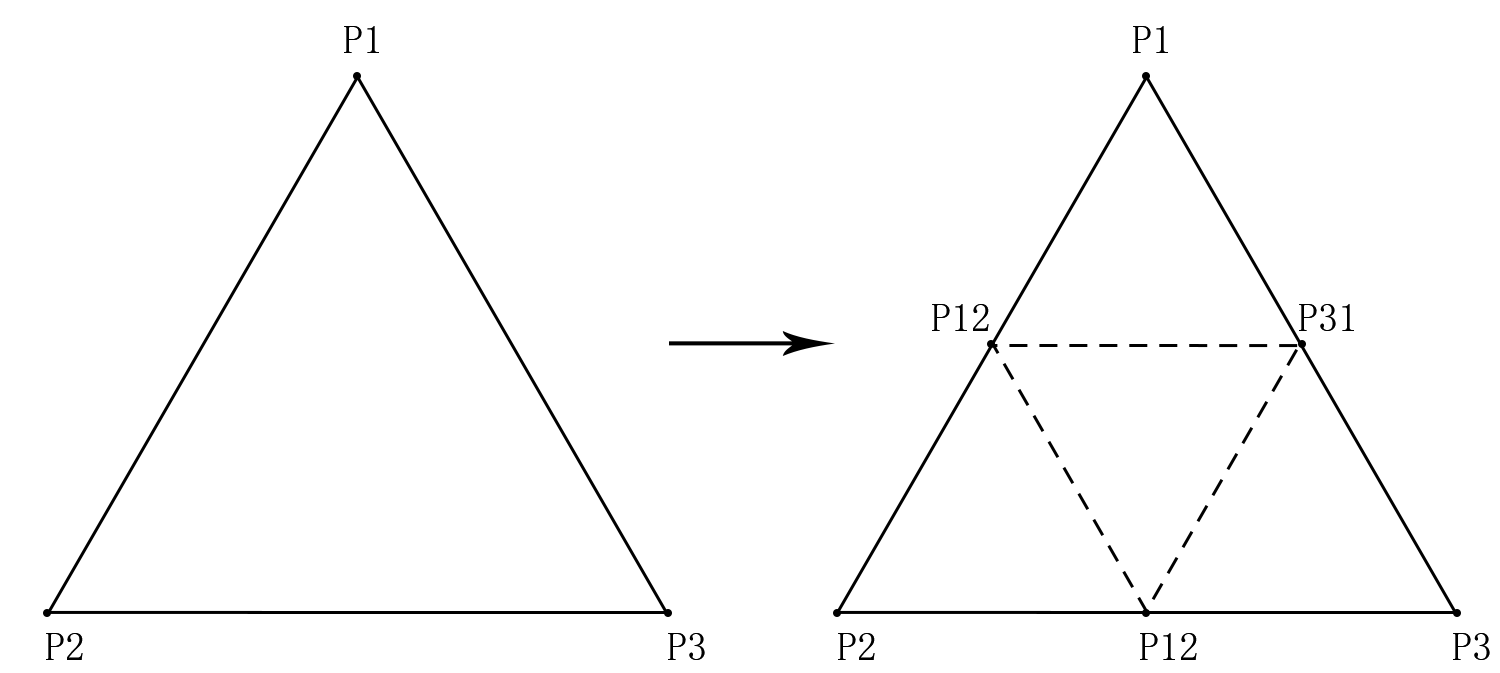
\includegraphics[width=0.75\linewidth]{./Figure/LinearSubdivision.png}
  \caption{Linear one to four subdivision for triangulars.}\label{Figure_Linear_Subdivision}
\end{figure}

Our proposed method implements linear one to four triangular mesh subdivisions to increase the details in a mesh as illustrated in Fig. \ref{Figure_Linear_Subdivision}, and then smooths it to accomplish surface approximation after subdivision while actualizing shape retention.

Denote the original mesh as $M_i$, and the edge point generator $G_{EFPMS}$ is depicted in Fig. \ref{Figure_Edge_Point_Generator}. To perform linear triangular subdivision, we insert points created by generator $G_{EFPMS}$ on the edge of each triangle to the hash map $H_n(v_i,h_i)$ for storing vertices $v_i$ and their handles $h_i$ as corresponding hash keys. For each vertex on mesh $\{v_1,v_2,\ldots,v_n\}$, we check whether the generated middle edge point $v_k$ is already in the map. If so, we get its handle $h_k$ for the on-coming face generation, and otherwise insert the point $v_k$ into the mesh and create its handle $h_k$ while updating vertices hash map $H_{n+1}(v_i,h_i)$. Finally, the new triangular surfaces are formed using vertex handles geometrically anticlockwise, and  older redundant faces are eliminated simultaneously. Each triangle will then be split into four sub-triangles and original mesh $M_i$ is subdivided to $M_{i+1}$. %Pseudocode of linear one to four subdivisions is illustrated in Algorithm \ref{Algorithm_Linear}.


%\begin{algorithm}
%    \caption{Linear Triangular Mesh Subdivision}
%    \label{Algorithm_Linear}
%    \hspace*{\algorithmicindent} \textbf{Input~~ : Original Mesh $M_i$} \\
%    \hspace*{\algorithmicindent} \textbf{Output~: Subdivided Mesh $M_{i+1}$} \\
%    \begin{algorithmic}
%        \FOR {\textbf{each} triangular face $f_i$ \textbf{in} $M_i$}
%            \STATE {get $3$ middle point on edges of $f_i$;}
%            \STATE {generate $4$ subfaces anticlockwise;}
%        \ENDFOR
%        \STATE {}
%    \end{algorithmic}
%\end{algorithm}

\begin{figure}[!htb]
  \centering
%  \captionsetup{justification=centering,margin=1cm}
  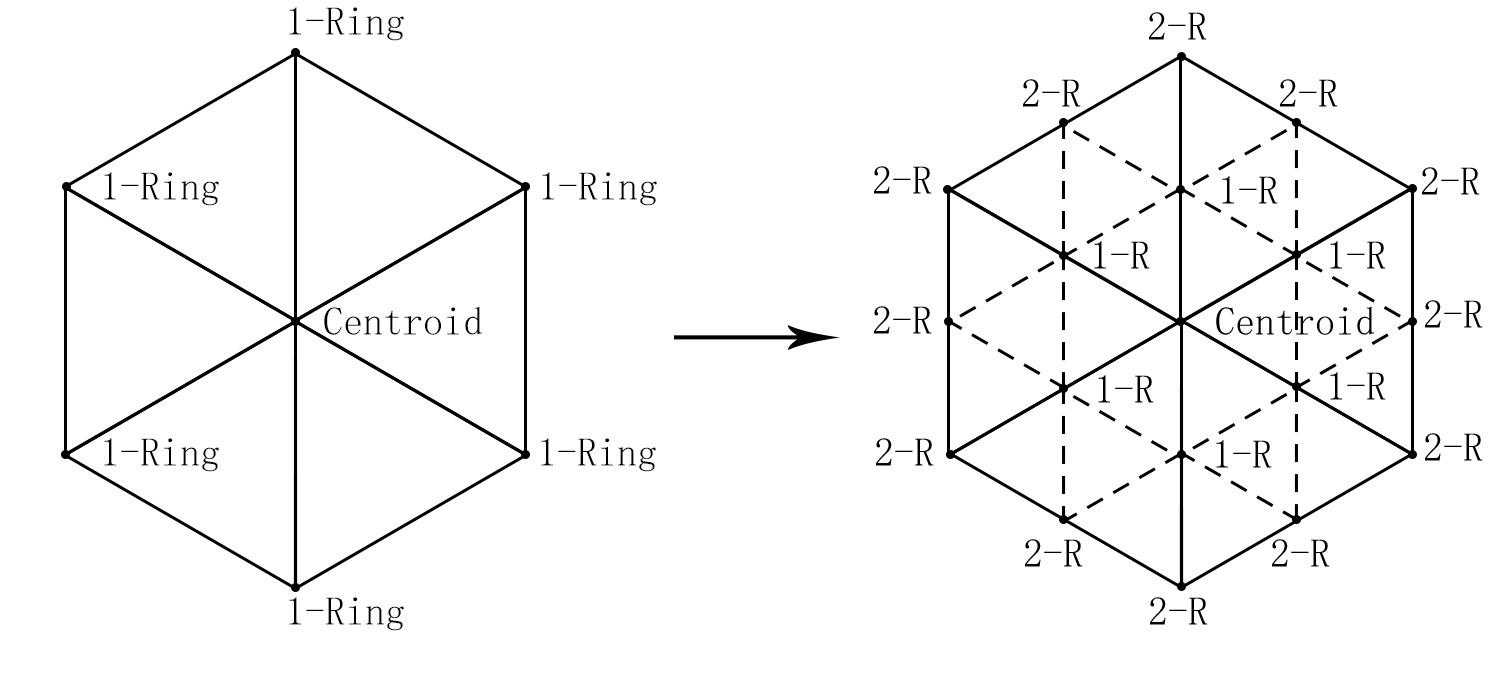
\includegraphics[width=0.9\linewidth]{./Figure/OneRingVerticesDerivative.png}
  \caption{One-ring vertices derivative.}\label{Figure_OneRing_Vertices_Derivative}
\end{figure}

\begin{figure}[htbp]
  \centering
%  \captionsetup{justification=centering,margin=0.5cm}
  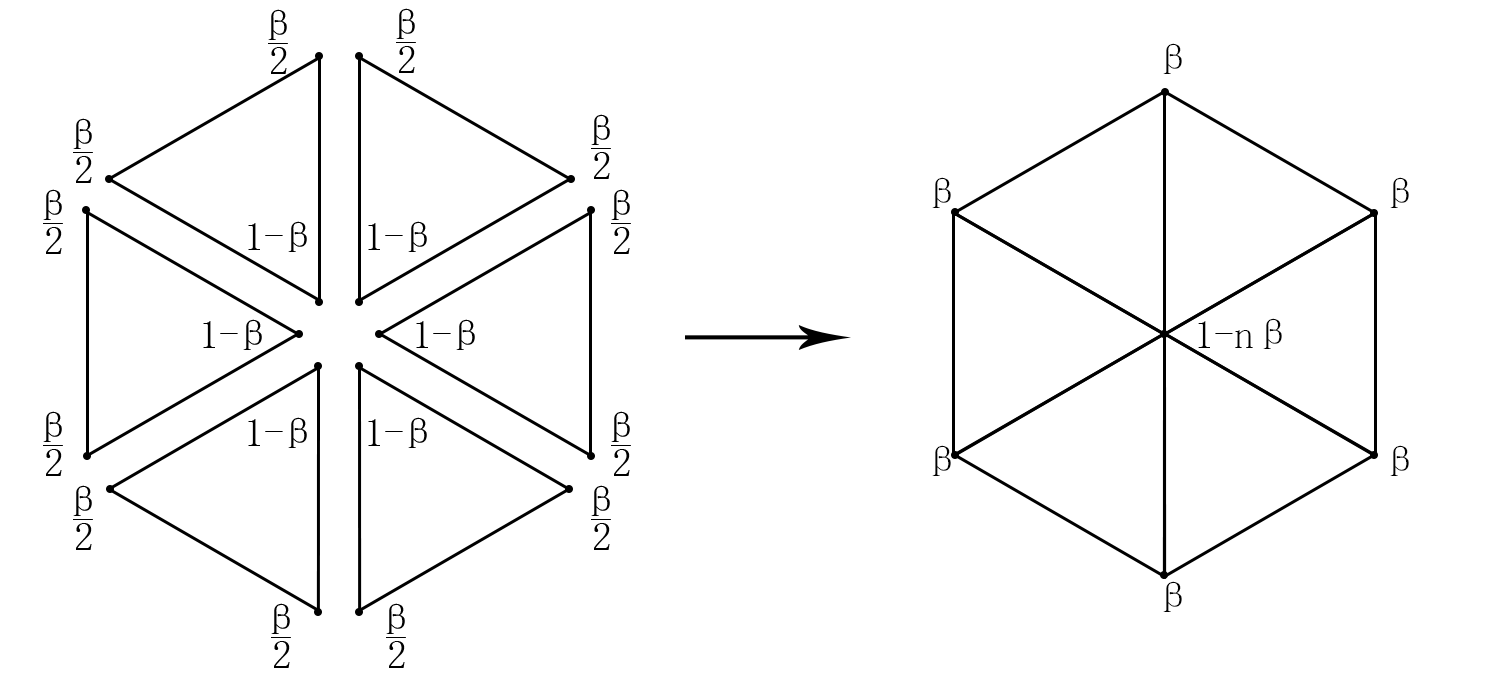
\includegraphics[width=0.9\linewidth]{./Figure/WeightedCentroid.png}
  \caption{One-ring neighbor weighted centroid method.}\label{Figure_Weighted_Centroid}
\end{figure}

Smoothing for triangular meshes will be applied to not only the previous vertices on $M_i$ but also all vertices on the generated mesh $M_{i+1}$ whose two-ring vertex set is derived from one-ring vertices of previous mesh $M_i$ as illustrated in Fig. \ref{Figure_OneRing_Vertices_Derivative}. For each vertex on $M_{i+1}$, we use a one-ring neighbor weighted centroid method for averaging as shown in Fig. \ref{Figure_Weighted_Centroid}. The weight of each neighbor $\beta$ is decided by the number of one-ring neighbors $n$:

\begin{equation}\label{Equation_beta}
  \beta=\frac{5}{8}-(\frac{3}{8}+\frac{1}{4}\cos\frac{2\pi}{n})^2
\end{equation}


\begin{figure*}[htbp]
  \centering
%  \captionsetup{justification=centering,margin=0.7cm}
  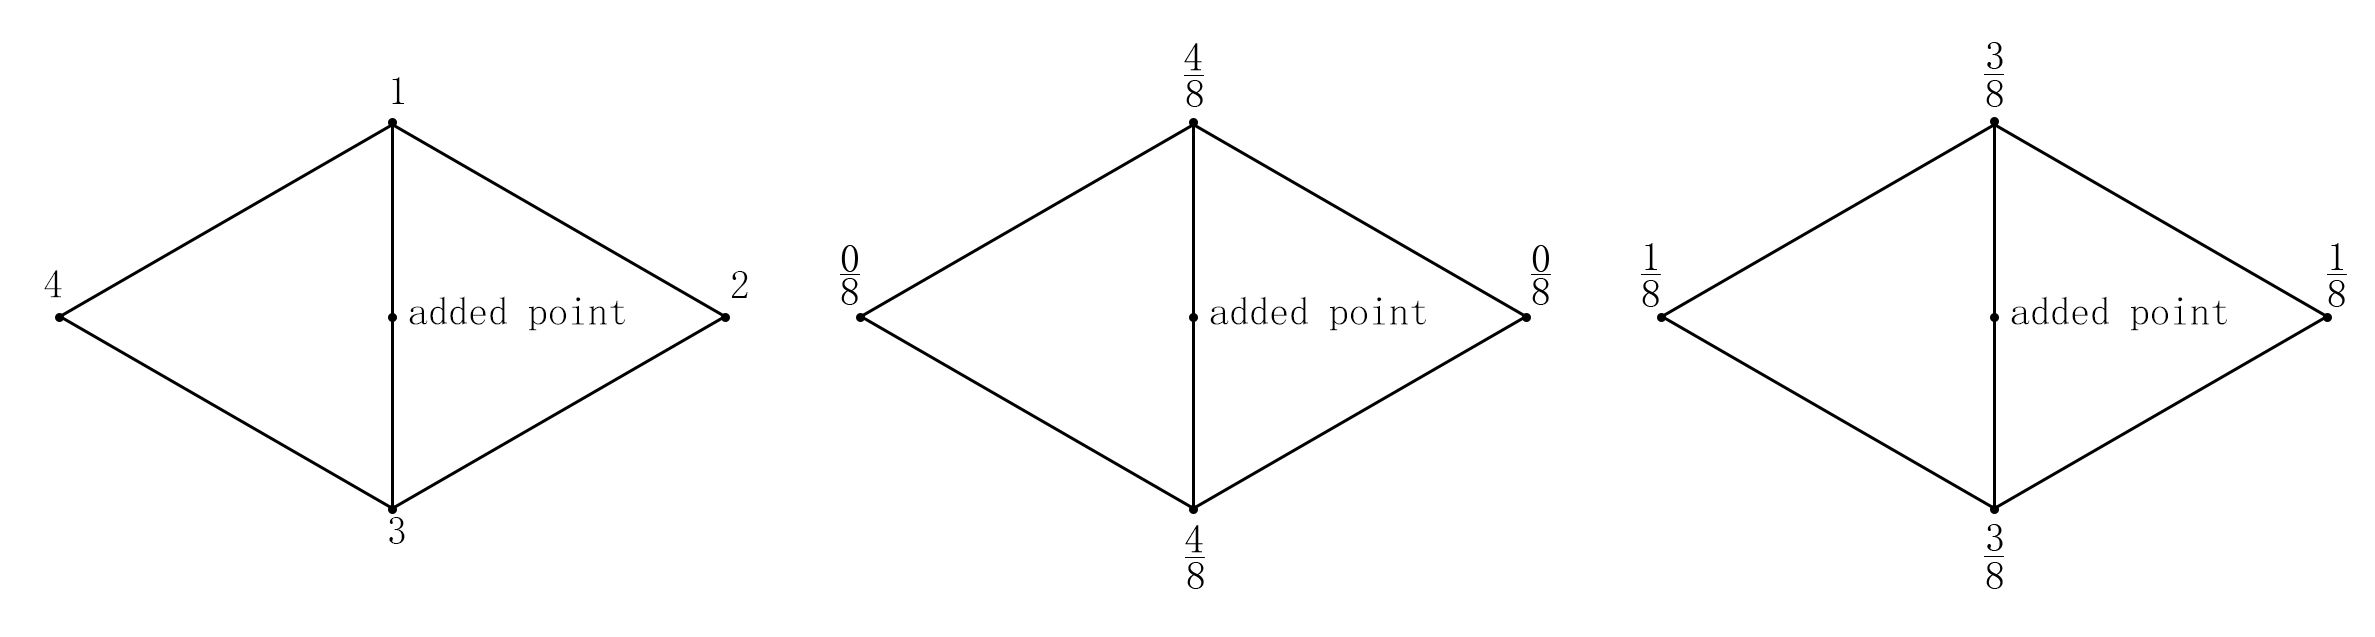
\includegraphics[width=0.9\linewidth]{./Figure/EdgePointGenerator.png}
  \caption{Unit of edge point generator (left). Feature Preserved Mesh Subdivision edge point generator (middle). Smoothness-focused Mesh Subdivision edge point generator (right). Weight of vertices in each generator are tagged aside its position.}\label{Figure_Edge_Point_Generator}
\end{figure*}

\begin{algorithm}
    \caption{Edge Feature Preserved Mesh Subdivision}
    \label{Algorithm_EFPMS}
    \hspace*{\algorithmicindent} \textbf{Input~~ : Original Mesh $M_i$} \\
    \hspace*{\algorithmicindent} \textbf{Output~: Subdivided Mesh $M_{i+1}$} \\
    \begin{algorithmic}
        \FOR {\textbf{each} triangular face $f_i$ \textbf{in} $M_i$}
            \STATE {get $3$ edge point on edges of $f_i$ with $G_{FPMS}$;}
            \STATE {generate $4$ subfaces anticlockwise;}
        \ENDFOR\\
        \COMMENT {NOTE: $M_i$ is now subdivided into $M_{i+1}$}
        \STATE {}
        \FOR {\textbf{each} vertex $v_i$ \textbf{in} $M_{i+1}$}
            \STATE {$N(v_i)$ = 1-ring neighbors of $v_i$ on current mesh $M_{i+1}$;}
            \STATE {$v_i$ = 1-ring Neighbor Weighted Centroid method on $v_i$;}
        \ENDFOR\\
        \COMMENT {NOTE: $M_{i+1}$ is now smoothed}
        \STATE {}
    \end{algorithmic}
\end{algorithm}

%%%%%%%%%%%%%%%%%%%%%%%%%%%%%%%%%%%%%%%%%%%%%%%%%%%%%%%%%%%%%%%%%%%%%%%%%%%%%%%%%%%%%%%%%%%%%%%%%%%%%%%%

\subsection{Model-dependent Wavelike Noise Elimination}
By using EFPMS, an edge and vertex aware result is generated. But the method will generate model-dependent wavelike noise on the mesh, as illustrated in Fig. \ref{Figure_Noise}.

\begin{figure}[htbp]
  \centering
%  \captionsetup{justification=centering,margin=0.2cm}

  \subfigure[]{
      \begin{minipage}[h]{0.48\linewidth}
        \centering
        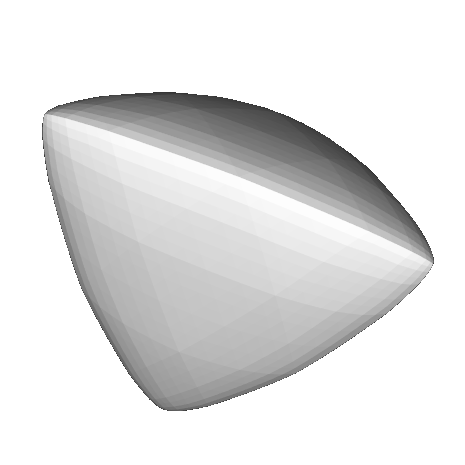
\includegraphics[width=\textwidth]{./Figure/tetrahedron/Noise.png}\\
      \end{minipage}
  }%
  \hskip -2ex
  \subfigure[]{
      \begin{minipage}[h]{0.48\linewidth}
        \centering
        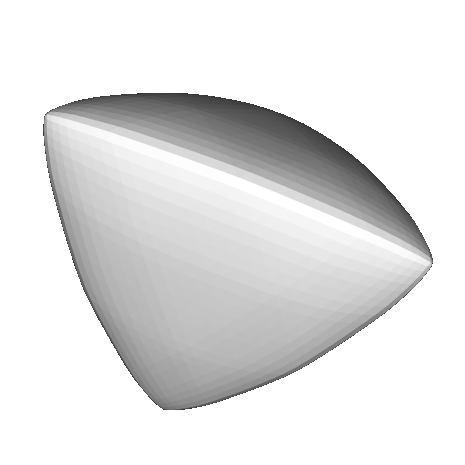
\includegraphics[width=\textwidth]{./Figure/tetrahedron/Noise-removed.png}\\
      \end{minipage}
  }

  \caption{a) Model-dependent wavelike noise. b) Removing wavelike noise by Smoothness-focused Mesh Subdivision. All subdivision algorithms have been applied five iterations on original meshes.}\label{Figure_Noise}
\end{figure}


We propose Model-dependent Wavelike Noise Elimination, a combination of EFPMS and Smoothness-focused Mesh Subdivision (SMS), to eliminate noise. The subdivision scheme consists of several iterations of EFPMS and an iteration of SMS at the end of the algorithm. %as illustrated in Algorithm \ref{Algorithm_SMS}.
The implementation of SMS resembles the EFPMS, except the generation of edge points and smoothing operator.

Unlike edge points generator $G_{EFPMS}$ in feature preserved subdivision, edge points in the last iteration of noise elimination algorithm are generated based on weighted neighbors illustrated in Fig. \ref{Figure_Edge_Point_Generator}, where directly connected vertices take up a greater weight, namely 3/8 each, and indirect weight is slightly less, namely 1/8 each.

Neighbor vertices in the smoothing method depend on previous one-ring vertices on $M_i$, but not newly generated vertices on $M_{i+1}$, which is different from the implementation of EFPMS. The weight of each neighbor follows the same principle introduced in EFPMS.

%\begin{algorithm}
%    \caption{Model-dependent Wavelike Noise Elimination}
%    \label{Algorithm_SMS}
%    \hspace*{\algorithmicindent} \textbf{Input~~ : Original Mesh $M_i$} \\
%    \hspace*{\algorithmicindent} \textbf{Output~: Subdivided Mesh $M_{i+1}$} \\
%    \begin{algorithmic}
%        \STATE {several iterations on EFPMS;}\\
%        \COMMENT {NOTE: oncoming is Smoothness-focused iteration}
%        \STATE {}
%        \FOR {\textbf{each} triangular face $f_i$ \textbf{in} $M_i$}
%            \STATE {get $3$ edge point on edges of $f_i$ with $G_{SMS}$;}
%            \STATE {generate $4$ subfaces anticlockwise;}
%        \ENDFOR\\
%        \COMMENT {NOTE: $M_i$ is now subdivided into $M_{i+1}$}
%        \STATE {}
%        \FOR {\textbf{each} vertex $v_i$ \textbf{in} $M_{i+1}$}
%            \STATE {$N(v_i)$ = 1-ring neighbors of $v_i$ on previous mesh $M_i$;}
%            \STATE {$v_i$ = 1-ring Neighbor Weighted Centroid method on $v_i$;}
%        \ENDFOR\\
%        \COMMENT {NOTE: $M_{i+1}$ is now smoothed}
%        \STATE {}
%    \end{algorithmic}
%\end{algorithm}

%%%%%%%%%%%%%%%%%%%%%%%%%%%%%%%%%%%%%%%%%%%%%%%%%%%%%%%%%%%%%%%%%%%%%%%%%%%%%%%%%%%%%%%%%%%%%%%%%%%%%%%%
%%%%%%%%%%%%%%%%%%%%%%%%%%%%%%%%%%%%%%%%%%%%%%%%%%%%%%%%%%%%%%%%%%%%%%%%%%%%%%%%%%%%%%%%%%%%%%%%%%%%%%%%

\section{Feature Preserved Mesh Subdivision Framework}\label{Section:Keypoint based Feature Preserved Mesh Subdivision Scheme}
In this section, we propose a Feature Preserved Mesh Subdivision Framework (FPMS), which contains edge point generation and smooth operator, to balance the emphasis of original features and smoothing extent. The big picture of our framework is using detected points to guide subdivision procedures. Based on imbalanced keypoint detection, all the vertices are classified into two categories, and keypoints are distributed mainly at the boundaries and detailed parts, which should be kept after subdivision but slightly adjusted with neighbors. The proposed FPMS framework is depicted in Algorithm \ref{Algorithm_FPMS}.

The unit of edge point generation in our provided method is a couple of triangles back to back as illustrated in Fig. \ref{Figure_Edge_Point_Generator}. Denote edge point generators in Edge Feature Preserved Mesh Subdivision and Smoothness-based Mesh Subdivision as $G_{EFPMS}(N)$ and $G_{SMS}(N)$ respectively, where $N$ is the set of neighbor points.


\begin{figure*}[htbp]
  \centering
%  \captionsetup{justification=centering,margin=1cm}

  \subfigure[Butterfly]{
      \begin{minipage}[h]{0.16\linewidth}
        \centering
        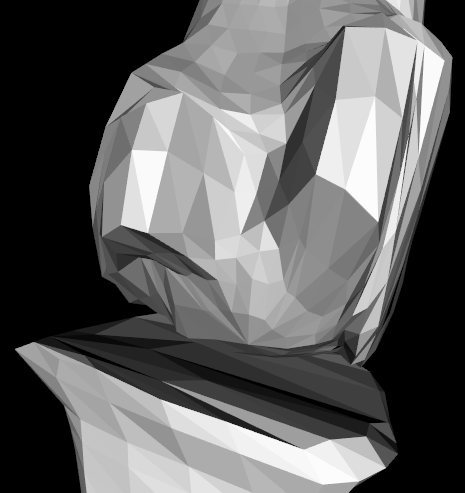
\includegraphics[width=\textwidth]{./Figure/footbones/fingerBones/butterfly1.png}\\
        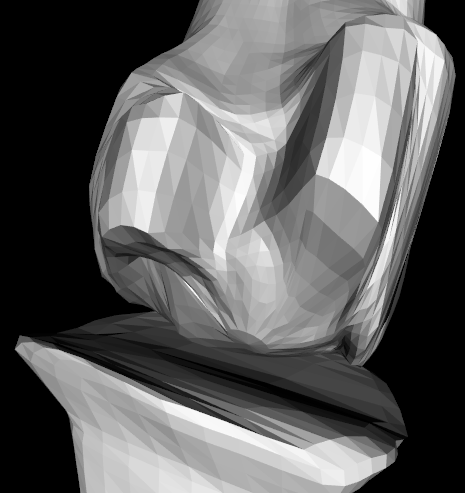
\includegraphics[width=\textwidth]{./Figure/footbones/fingerBones/butterfly2.png}\\
        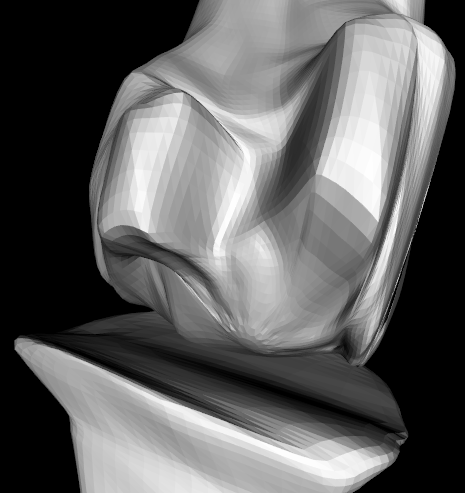
\includegraphics[width=\textwidth]{./Figure/footbones/fingerBones/butterfly3.png}\vspace{1ex}\\
      \end{minipage}%
      \begin{minipage}[h]{0.16\linewidth}
        \centering
        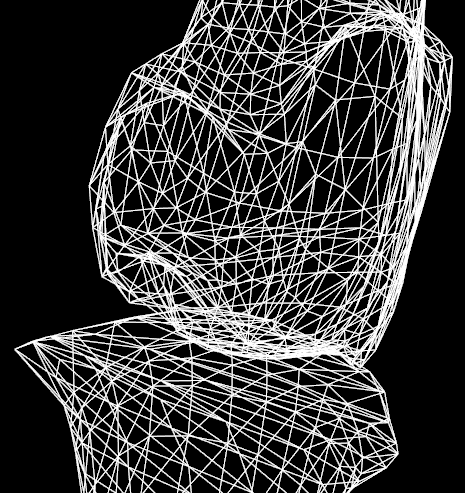
\includegraphics[width=\textwidth]{./Figure/footbones/fingerBones/butterfly1-.png}\\
        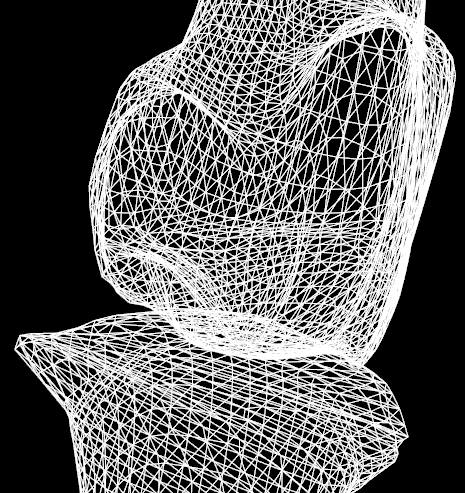
\includegraphics[width=\textwidth]{./Figure/footbones/fingerBones/butterfly2-.png}\\
        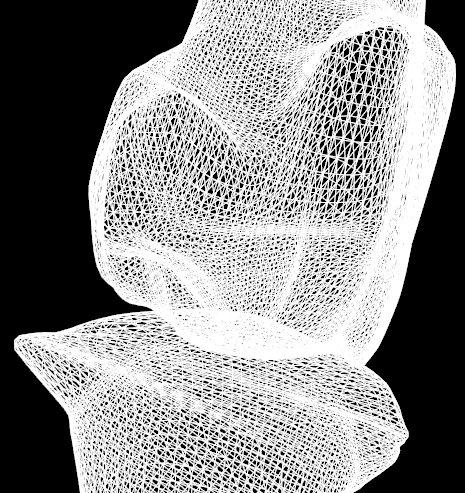
\includegraphics[width=\textwidth]{./Figure/footbones/fingerBones/butterfly3-.png}\vspace{1ex}\\
      \end{minipage}
  }
  \hskip -1ex
  \subfigure[Catmull]{
      \begin{minipage}[h]{0.16\linewidth}
        \centering
        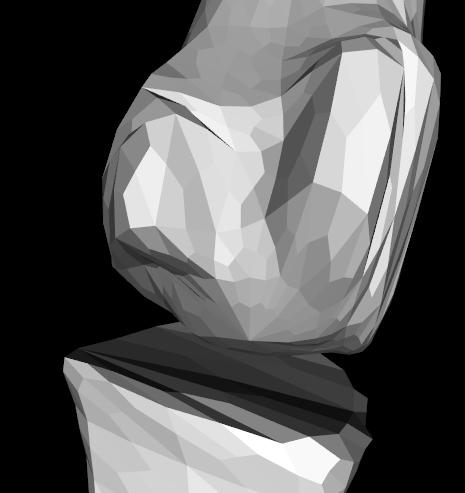
\includegraphics[width=\textwidth]{./Figure/footbones/fingerBones/catmull1.png}\\
        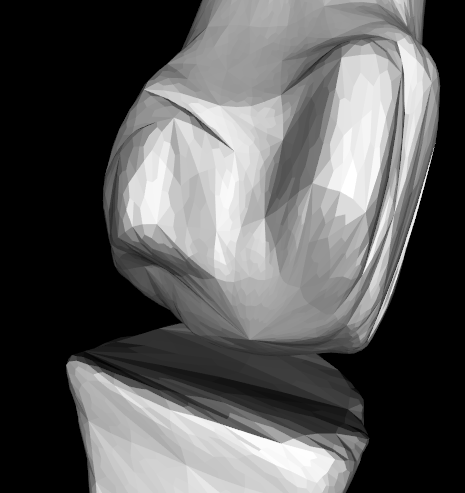
\includegraphics[width=\textwidth]{./Figure/footbones/fingerBones/catmull2.png}\\
        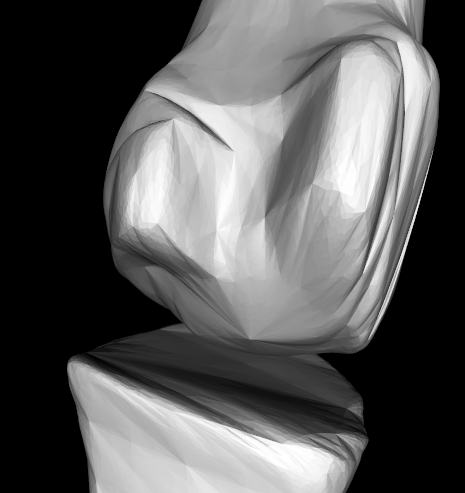
\includegraphics[width=\textwidth]{./Figure/footbones/fingerBones/catmull3.png}\vspace{1ex}\\
      \end{minipage}%
      \begin{minipage}[h]{0.16\linewidth}
        \centering
        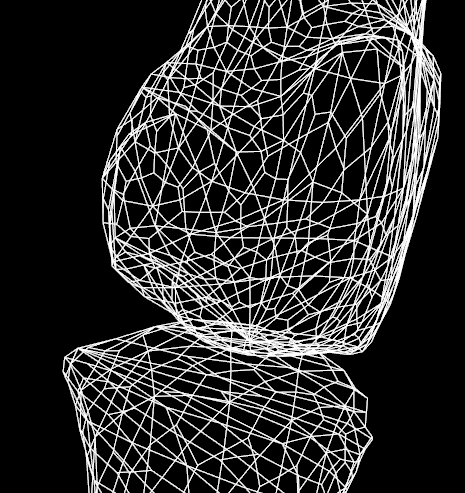
\includegraphics[width=\textwidth]{./Figure/footbones/fingerBones/catmull1-.png}\\
        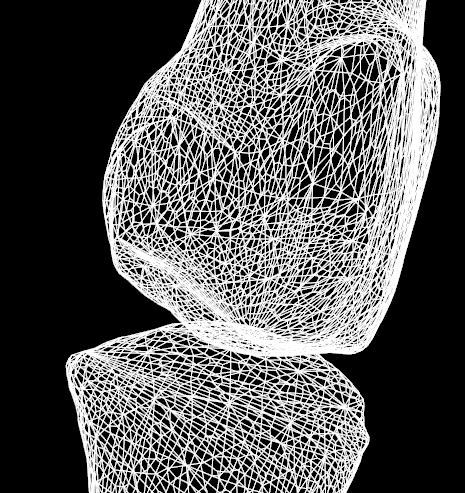
\includegraphics[width=\textwidth]{./Figure/footbones/fingerBones/catmull2-.png}\\
        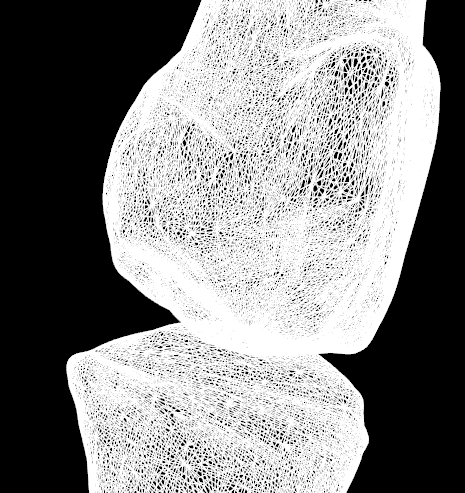
\includegraphics[width=\textwidth]{./Figure/footbones/fingerBones/catmull3-.png}\vspace{1ex}\\
      \end{minipage}
  }
  \hskip -1ex
  \subfigure[Loop]{
      \begin{minipage}[h]{0.16\linewidth}
        \centering
        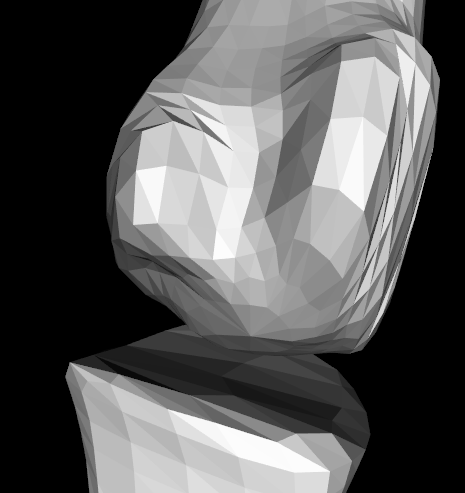
\includegraphics[width=\textwidth]{./Figure/footbones/fingerBones/loop1.png}\\
        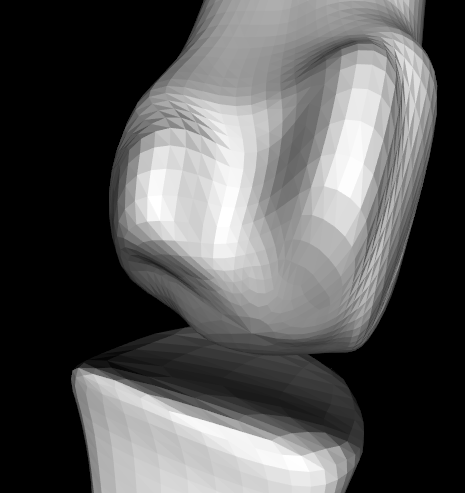
\includegraphics[width=\textwidth]{./Figure/footbones/fingerBones/loop2.png}\\
        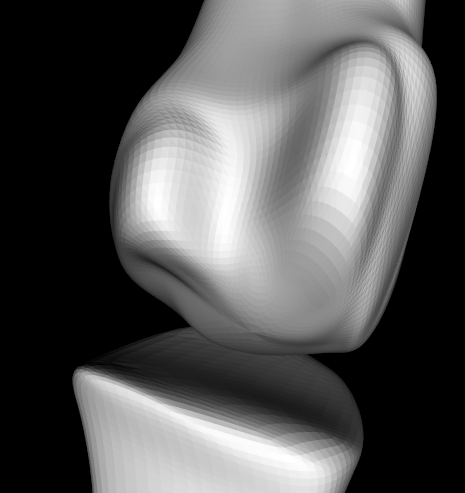
\includegraphics[width=\textwidth]{./Figure/footbones/fingerBones/loop3.png}\vspace{1ex}\\
      \end{minipage}%
      \begin{minipage}[h]{0.16\linewidth}
        \centering
        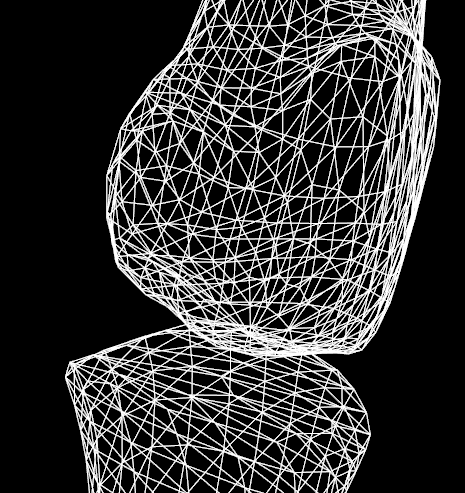
\includegraphics[width=\textwidth]{./Figure/footbones/fingerBones/loop1-.png}\\
        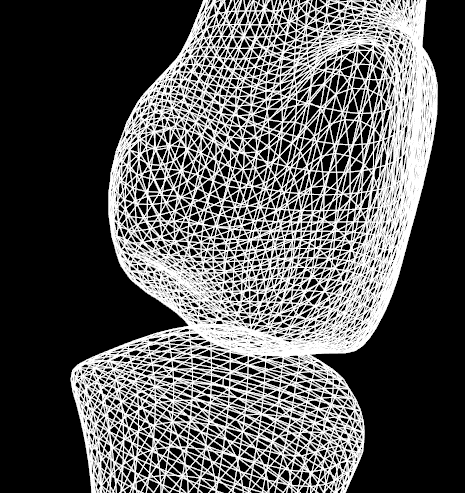
\includegraphics[width=\textwidth]{./Figure/footbones/fingerBones/loop2-.png}\\
        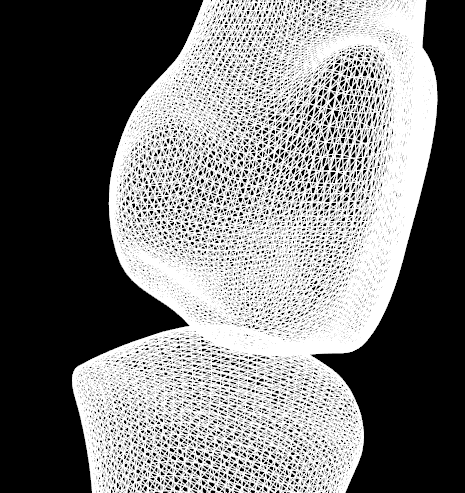
\includegraphics[width=\textwidth]{./Figure/footbones/fingerBones/loop3-.png}\vspace{1ex}\\
      \end{minipage}
  }
  \hskip -1ex
  \subfigure[EFPMS]{
      \begin{minipage}[h]{0.16\linewidth}
        \centering
        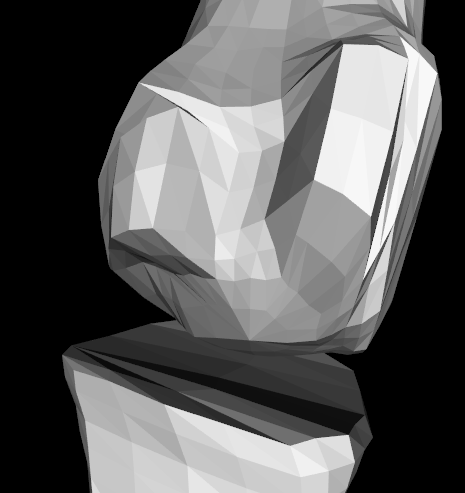
\includegraphics[width=\textwidth]{./Figure/footbones/fingerBones/weight21.png}\\
        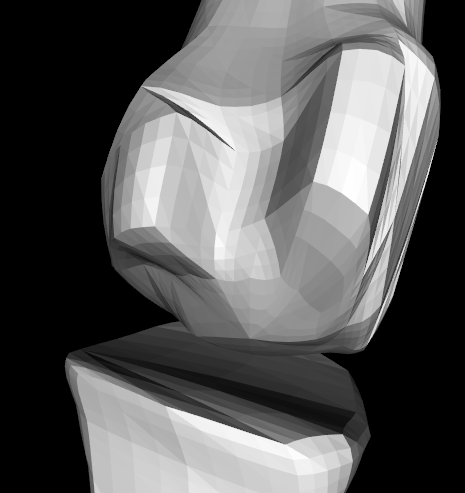
\includegraphics[width=\textwidth]{./Figure/footbones/fingerBones/weight22.png}\\
        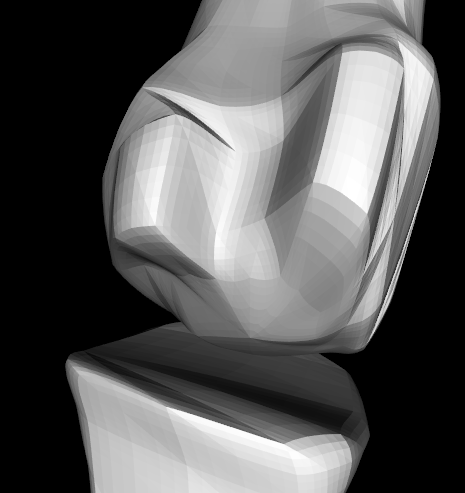
\includegraphics[width=\textwidth]{./Figure/footbones/fingerBones/weight23.png}\vspace{1ex}\\
      \end{minipage}%
      \begin{minipage}[h]{0.16\linewidth}
        \centering
        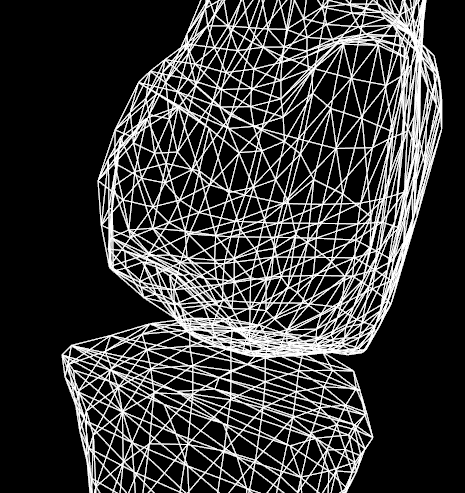
\includegraphics[width=\textwidth]{./Figure/footbones/fingerBones/weight21-.png}\\
        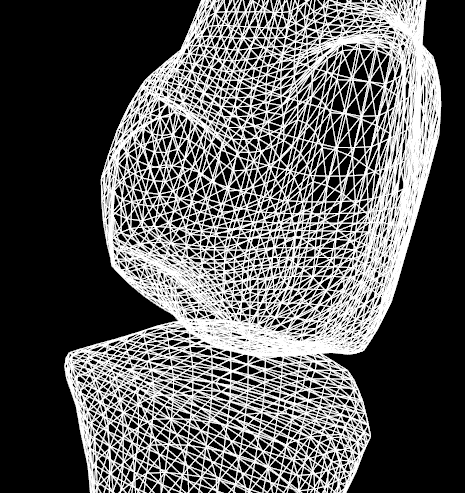
\includegraphics[width=\textwidth]{./Figure/footbones/fingerBones/weight22-.png}\\
        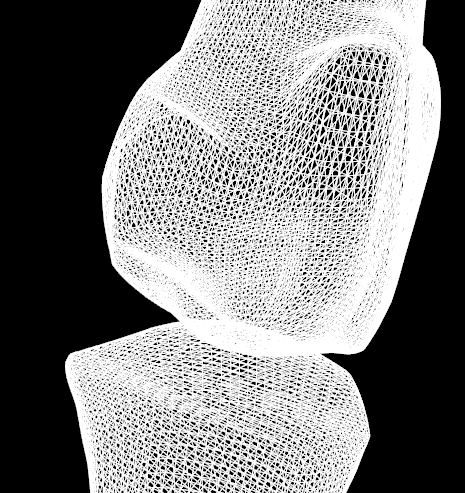
\includegraphics[width=\textwidth]{./Figure/footbones/fingerBones/weight23-.png}\vspace{1ex}\\
      \end{minipage}
  }
  \hskip -1ex
  \subfigure[SMS]{
      \begin{minipage}[h]{0.16\linewidth}
        \centering
        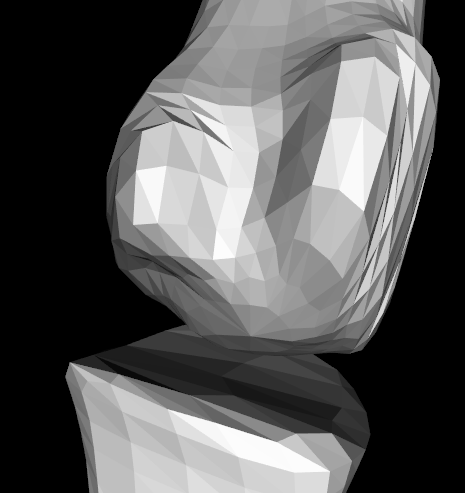
\includegraphics[width=\textwidth]{./Figure/footbones/fingerBones/combined1.png}\\
        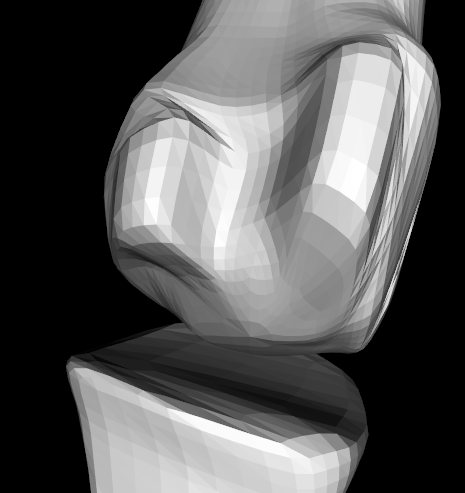
\includegraphics[width=\textwidth]{./Figure/footbones/fingerBones/combined2.png}\\
        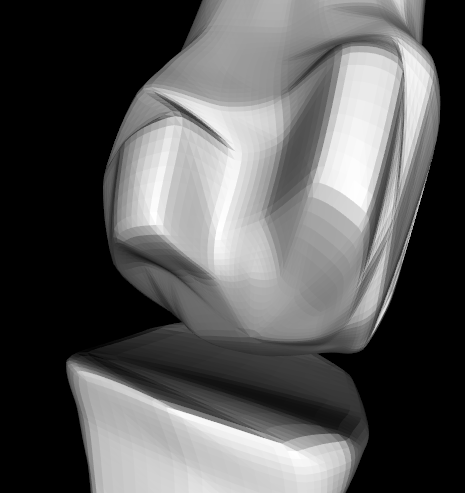
\includegraphics[width=\textwidth]{./Figure/footbones/fingerBones/combined3.png}\vspace{1ex}\\
      \end{minipage}%
      \begin{minipage}[h]{0.16\linewidth}
        \centering
        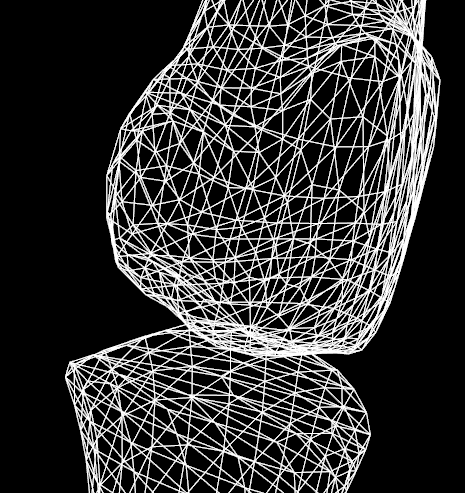
\includegraphics[width=\textwidth]{./Figure/footbones/fingerBones/combined1-.png}\\
        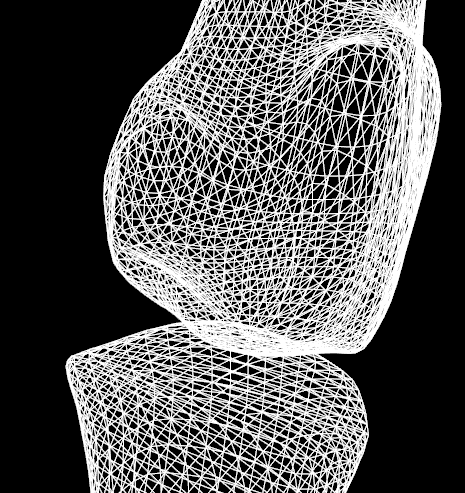
\includegraphics[width=\textwidth]{./Figure/footbones/fingerBones/combined2-.png}\\
        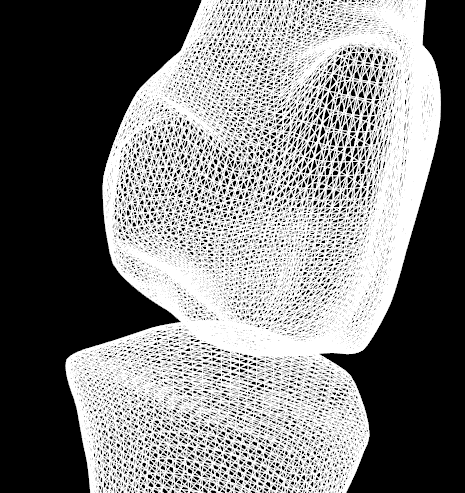
\includegraphics[width=\textwidth]{./Figure/footbones/fingerBones/combined3-.png}\vspace{1ex}\\
      \end{minipage}
  }
  \hskip -1ex
  \subfigure[FPMS]{
      \begin{minipage}[h]{0.16\linewidth}
        \centering
        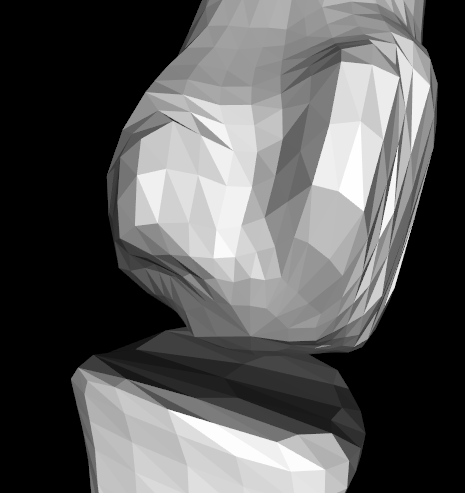
\includegraphics[width=\textwidth]{./Figure/footbones/fingerBones/kpw1.png}\\
        \includegraphics[width=\textwidth]{./Figure/footbones/fingerBones/kpw2.png}\\
        \includegraphics[width=\textwidth]{./Figure/footbones/fingerBones/kpw3.png}\vspace{1ex}\\
      \end{minipage}%
      \begin{minipage}[h]{0.16\linewidth}
        \centering
        \includegraphics[width=\textwidth]{./Figure/footbones/fingerBones/kpw1-.png}\\
        \includegraphics[width=\textwidth]{./Figure/footbones/fingerBones/kpw2-.png}\\
        \includegraphics[width=\textwidth]{./Figure/footbones/fingerBones/kpw3-.png}\vspace{1ex}\\
      \end{minipage}
  }

  \caption{Subdivision Comparison on phalangeals with iteration increasing by rows. a) Butterfly Method. b) Catmull Method. c) Loop Method. d) Edge Feature Preserved Mesh Subdivision. e) Smoothness-focused Mesh Subdivision. f) Feature Preserved Mesh Subdivision.}\label{Figure_KFPMS_1}
\end{figure*}



\begin{figure*}[htbp]
  \centering
%  \captionsetup{justification=centering,margin=1cm}

  \subfigure[Butterfly]{
      \begin{minipage}[h]{0.16\linewidth}
        \centering
        \includegraphics[width=\textwidth]{./Figure/footbones/middle/butterfly1.png}\\
        \includegraphics[width=\textwidth]{./Figure/footbones/middle/butterfly2.png}\\
        \includegraphics[width=\textwidth]{./Figure/footbones/middle/butterfly3.png}\vspace{1ex}\\
      \end{minipage}
  }%
  \hskip -2ex
  \subfigure[Catmull]{
      \begin{minipage}[h]{0.16\linewidth}
        \centering
        \includegraphics[width=\textwidth]{./Figure/footbones/middle/catmull1.png}\\
        \includegraphics[width=\textwidth]{./Figure/footbones/middle/catmull2.png}\\
        \includegraphics[width=\textwidth]{./Figure/footbones/middle/catmull3.png}\vspace{1ex}\\
      \end{minipage}
  }%
  \hskip -2ex
  \subfigure[Loop]{
      \begin{minipage}[h]{0.16\linewidth}
        \centering
        \includegraphics[width=\textwidth]{./Figure/footbones/middle/loop1.png}\\
        \includegraphics[width=\textwidth]{./Figure/footbones/middle/loop2.png}\\
        \includegraphics[width=\textwidth]{./Figure/footbones/middle/loop3.png}\vspace{1ex}\\
      \end{minipage}
  }%
  \hskip -2ex
  \subfigure[EFPMS]{
      \begin{minipage}[h]{0.16\linewidth}
        \centering
        \includegraphics[width=\textwidth]{./Figure/footbones/middle/weight21.png}\\
        \includegraphics[width=\textwidth]{./Figure/footbones/middle/weight22.png}\\
        \includegraphics[width=\textwidth]{./Figure/footbones/middle/weight23.png}\vspace{1ex}\\
      \end{minipage}
  }%
  \hskip -2ex
  \subfigure[SMS]{
      \begin{minipage}[h]{0.16\linewidth}
        \centering
        \includegraphics[width=\textwidth]{./Figure/footbones/middle/combined1.png}\\
        \includegraphics[width=\textwidth]{./Figure/footbones/middle/combined2.png}\\
        \includegraphics[width=\textwidth]{./Figure/footbones/middle/combined3.png}\vspace{1ex}\\
      \end{minipage}
  }%
  \hskip -2ex
  \subfigure[FPMS]{
      \begin{minipage}[h]{0.16\linewidth}
        \centering
        \includegraphics[width=\textwidth]{./Figure/footbones/middle/kpw1.png}\\
        \includegraphics[width=\textwidth]{./Figure/footbones/middle/kpw2.png}\\
        \includegraphics[width=\textwidth]{./Figure/footbones/middle/kpw3.png}\vspace{1ex}\\
      \end{minipage}
  }

  \caption{Subdivision Comparison on human footbone with iteration increasing by rows. a) Butterfly Method. b) Catmull Method. c) Loop Method. d) Edge Feature Preserved Mesh Subdivision. e) Smoothness-focused Mesh Subdivision. f) Feature Preserved Mesh Subdivision.}\label{Figure_KFPMS_2}
\end{figure*}

\begin{figure*}[htbp]
  \centering
%  \captionsetup{justification=centering,margin=1cm}

  \subfigure[Butterfly]{
      \begin{minipage}[h]{0.16\linewidth}
        \centering
        \includegraphics[width=\textwidth]{./Figure/footbones/end/butterfly1.png}\\
        \includegraphics[width=\textwidth]{./Figure/footbones/end/butterfly2.png}\\
        \includegraphics[width=\textwidth]{./Figure/footbones/end/butterfly3.png}\vspace{1ex}\\
      \end{minipage}
  }%
  \hskip -2ex
  \subfigure[Catmull]{
      \begin{minipage}[h]{0.16\linewidth}
        \centering
        \includegraphics[width=\textwidth]{./Figure/footbones/end/catmull1.png}\\
        \includegraphics[width=\textwidth]{./Figure/footbones/end/catmull2.png}\\
        \includegraphics[width=\textwidth]{./Figure/footbones/end/catmull3.png}\vspace{1ex}\\
      \end{minipage}
  }%
  \hskip -2ex
  \subfigure[Loop]{
      \begin{minipage}[h]{0.16\linewidth}
        \centering
        \includegraphics[width=\textwidth]{./Figure/footbones/end/loop1.png}\\
        \includegraphics[width=\textwidth]{./Figure/footbones/end/loop2.png}\\
        \includegraphics[width=\textwidth]{./Figure/footbones/end/loop3.png}\vspace{1ex}\\
      \end{minipage}
  }%
  \hskip -2ex
  \subfigure[EFPMS]{
      \begin{minipage}[h]{0.16\linewidth}
        \centering
        \includegraphics[width=\textwidth]{./Figure/footbones/end/weight21.png}\\
        \includegraphics[width=\textwidth]{./Figure/footbones/end/weight22.png}\\
        \includegraphics[width=\textwidth]{./Figure/footbones/end/weight23.png}\vspace{1ex}\\
      \end{minipage}
  }%
  \hskip -2ex
  \subfigure[SMS]{
      \begin{minipage}[h]{0.16\linewidth}
        \centering
        \includegraphics[width=\textwidth]{./Figure/footbones/end/combined1.png}\\
        \includegraphics[width=\textwidth]{./Figure/footbones/end/combined2.png}\\
        \includegraphics[width=\textwidth]{./Figure/footbones/end/combined3.png}\vspace{1ex}\\
      \end{minipage}
  }%
  \hskip -2ex
  \subfigure[FPMS]{
      \begin{minipage}[h]{0.16\linewidth}
        \centering
        \includegraphics[width=\textwidth]{./Figure/footbones/end/kpw1.png}\\
        \includegraphics[width=\textwidth]{./Figure/footbones/end/kpw2.png}\\
        \includegraphics[width=\textwidth]{./Figure/footbones/end/kpw3.png}\vspace{1ex}\\
      \end{minipage}
  }

  \caption{Subdivision Comparison on metatarsal bones and entocuneiforms with iteration increasing by rows. a) Butterfly Method. b) Catmull Method. c) Loop Method. d) Edge Feature Preserved Mesh Subdivision. e) Smoothness-focused Mesh Subdivision. f) Feature Preserved Mesh Subdivision.}\label{Figure_KFPMS_3}
\end{figure*}

The balance can be guided by the amount of imbalanced keypoints in an isolated generation unit and implemented by a weighted combination of $G_{EFPMS}(N)$ and $G_{SMS}(N)$. For a precise and accurate calculation, the weight of two generators should be geometrically related and symmetric. The weight of $G_{EFPMS}(N)$ and $G_{SMS}(N)$ will be defined as $W_{G_{EFPMS}}$ and $W_{G_{SMS}}$, which depend on the number of keypoints in a generation unit, and obey the following principles.

\begin{equation}\label{Equation_W_G_EFPMS}
  W_{G_{EFPMS}}=\sum_{i=1}^{|N|}{Key(N_i)}
\end{equation}

\begin{equation}\label{Equation_W_G_SMS}
  W_{G_{SMS}}=|N|-\sum_{i=1}^{|N|}{Key(N_i)}
\end{equation}

\begin{equation}\label{Equation_Key}
  Key(N_i)=
    \begin{cases}
    1& \text{$N_i$ is a keypoint} \\
    0& \text{else}
    \end{cases}
\end{equation}

A combination of two edge point generator $G(N)$ will be defined as:
\begin{equation}\label{Equation_G}
  G(N)=W_{G_{EFPMS}}G_{EFPMS}(N)+W_{G_{SMS}}G_{SMS}(N)
\end{equation}

Smooth operator will also be guided by keypoints, which extends the previous smoothing scheme. Neighbor vertices for smooth operator will be different, which depend on whether the centroid vertex is a keypoint or not. If so, neighbor vertices should be older one-ring vertices on $M_i$, and otherwise, one-ring vertices on $M_{i+1}$.

\begin{algorithm}
    \caption{Feature Preserved Mesh Subdivision}
    \label{Algorithm_FPMS}
    \hspace*{\algorithmicindent} \textbf{Input~~ : Original Mesh $M_i$} \\
    \hspace*{\algorithmicindent} \textbf{Output~: Subdivided Mesh $M_{i+1}$} \\
    \begin{algorithmic}
        \STATE {imbalanced keypoint detection on $M_i$;}\\
        \COMMENT {NOTE: vertices have been classified into two class}
        \STATE {}
        \FOR {\textbf{each} triangular face $f_i$ \textbf{in} $M_i$}
            \STATE {get edge point $e_{EFPMS}$ on edges of $f_i$ with $G_{EFPMS}$;}
            \STATE {get edge point $e_{SMS}$ on edges of $f_i$ with $G_{SMS}$;}
            \STATE {average position of edge points by $G(N)$;}
            \STATE {generate $4$ sub-faces anticlockwise;}
        \ENDFOR\\
        \COMMENT {NOTE: $M_i$ is now subdivided into $M_{i+1}$}
        \STATE {}
        \FOR {\textbf{each} vertex $v_i$ \textbf{in} $M_{i+1}$}
            \IF {$v_i$ is a keypoint}
                \STATE {$N(v_i)$ = 1-ring neighbors of $v_i$ on $M_i$;}
                \STATE {$v_i$ = 1-ring Neighbor Weighted Centroid on $v_i$;}
            \ELSE
                \STATE {$N(v_i)$ = 1-ring neighbors of $v_i$ on $M_{i+1}$;}
                \STATE {$v_i$ = 1-ring Neighbor Weighted Centroid on $v_i$;}
            \ENDIF
        \ENDFOR\\
        \COMMENT {NOTE: $M_{i+1}$ is now smoothed}
        \STATE {}
    \end{algorithmic}
\end{algorithm}

%%%%%%%%%%%%%%%%%%%%%%%%%%%%%%%%%%%%%%%%%%%%%%%%%%%%%%%%%%%%%%%%%%%%%%%%%%%%%%%%%%%%%%%%%%%%%%%%%%%%%%%%
%%%%%%%%%%%%%%%%%%%%%%%%%%%%%%%%%%%%%%%%%%%%%%%%%%%%%%%%%%%%%%%%%%%%%%%%%%%%%%%%%%%%%%%%%%%%%%%%%%%%%%%%

\section{Experiments}\label{Section:Experiment}
We test different subdivision methods on several biomedical data, including phalanx,
%(distal phalanx, middle phalanx, and proximal phalanx),
cuneiform bone,
%(intermediate cuneiform bones, entocuneiform, ectocuneiform),
central anlrle bone, cuboid bone, etc.

As the iteration number of subdivision methods increases, the performance of different algorithms becomes easier to differentiate, as illustrated in Fig. \ref{Figure_KFPMS_1}. Except Catmull method, all the subdivision methods implement one to four triangular subdivision, which means each mesh in a row has the same number of vertices and faces except the mesh generated by Catmull subdivision. The number of vertices and triangular faces in each iteration follows the below principles when applying one to four mesh subdivision schemes, where $V(\cdot)$ and $F(\cdot)$ represent total amount of vertices and faces on a mesh, respectively.

\begin{equation}\label{Equation_V}
  V(M_{i+1})=V(M_i)+\frac{3}{2}F(M_i)
\end{equation}

\begin{equation}\label{Equation_F}
  F(M_{i+1})=4F(M_i)
\end{equation}

Obviously, the subdivision result of Loop method has a better sphere-like appearance, while EFPMS provides a better property of edge feature preservation. Butterfly subdivision leads the resulted mesh to a more boundary malleable shape, while Catmull presents more vertex details. Model-dependent Wavelike Noise Elimination accomplishes an edge feature preservation and smooth result, but compared with FPMS, the latter provides a better result on both edge and vertex features.

Fig. \ref{Figure_KFPMS_2} and Fig. \ref{Figure_KFPMS_3} exhibit more experimental comparisons on different meshes of biomedical utilizations. As illustrated in the figures, our proposed framework accomplishes a better result.

%%%%%%%%%%%%%%%%%%%%%%%%%%%%%%%%%%%%%%%%%%%%%%%%%%%%%%%%%%%%%%%%%%%%%%%%%%%%%%%%%%%%%%%%%%%%%%%%%%%%%%%%
%%%%%%%%%%%%%%%%%%%%%%%%%%%%%%%%%%%%%%%%%%%%%%%%%%%%%%%%%%%%%%%%%%%%%%%%%%%%%%%%%%%%%%%%%%%%%%%%%%%%%%%%


% An example of a floating figure using the graphicx package.
% Note that \label must occur AFTER (or within) \caption.
% For figures, \caption should occur after the \includegraphics.
% Note that IEEEtran v1.7 and later has special internal code that
% is designed to preserve the operation of \label within \caption
% even when the captionsoff option is in effect. However, because
% of issues like this, it may be the safest practice to put all your
% \label just after \caption rather than within \caption{}.
%
% Reminder: the "draftcls" or "draftclsnofoot", not "draft", class
% option should be used if it is desired that the figures are to be
% displayed while in draft mode.
%
%\begin{figure}[!t]
%\centering
%\includegraphics[width=2.5in]{myfigure}
% where an .eps filename suffix will be assumed under latex,
% and a .pdf suffix will be assumed for pdflatex; or what has been declared
% via \DeclareGraphicsExtensions.
%\caption{Simulation Results}
%\label{fig_sim}
%\end{figure}

% Note that IEEE typically puts floats only at the top, even when this
% results in a large percentage of a column being occupied by floats.


% An example of a double column floating figure using two subfigures.
% (The subfig.sty package must be loaded for this to work.)
% The subfigure \label commands are set within each subfloat command, the
% \label for the overall figure must come after \caption.
% \hfil must be used as a separator to get equal spacing.
% The subfigure.sty package works much the same way, except \subfigure is
% used instead of \subfloat.
%
%\begin{figure*}[!t]
%\centerline{\subfloat[Case I]\includegraphics[width=2.5in]{subfigcase1}%
%\label{fig_first_case}}
%\hfil
%\subfloat[Case II]{\includegraphics[width=2.5in]{subfigcase2}%
%\label{fig_second_case}}}
%\caption{Simulation results}
%\label{fig_sim}
%\end{figure*}
%
% Note that often IEEE papers with subfigures do not employ subfigure
% captions (using the optional argument to \subfloat), but instead will
% reference/describe all of them (a), (b), etc., within the main caption.


% An example of a floating table. Note that, for IEEE style tables, the
% \caption command should come BEFORE the table. Table text will default to
% \footnotesize as IEEE normally uses this smaller font for tables.
% The \label must come after \caption as always.
%
%\begin{table}[!t]
%% increase table row spacing, adjust to taste
%\renewcommand{\arraystretch}{1.3}
% if using array.sty, it might be a good idea to tweak the value of
% \extrarowheight as needed to properly center the text within the cells
%\caption{An Example of a Table}
%\label{table_example}
%\centering
%% Some packages, such as MDW tools, offer better commands for making tables
%% than the plain LaTeX2e tabular which is used here.
%\begin{tabular}{|c||c|}
%\hline
%One & Two\\
%\hline
%Three & Four\\
%\hline
%\end{tabular}
%\end{table}


% Note that IEEE does not put floats in the very first column - or typically
% anywhere on the first page for that matter. Also, in-text middle ("here")
% positioning is not used. Most IEEE journals/conferences use top floats
% exclusively. Note that, LaTeX2e, unlike IEEE journals/conferences, places
% footnotes above bottom floats. This can be corrected via the \fnbelowfloat
% command of the stfloats package.

%%%%%%%%%%%%%%%%%%%%%%%%%%%%%%%%%%%%%%%%%%%%%%%%%%%%%%%%%%%%%%%%%%%%%%%%%%%%%%%%%%%%%%%%%%%%%%%%%%%%%%%%
%%%%%%%%%%%%%%%%%%%%%%%%%%%%%%%%%%%%%%%%%%%%%%%%%%%%%%%%%%%%%%%%%%%%%%%%%%%%%%%%%%%%%%%%%%%%%%%%%%%%%%%%


\section{Conclusion}\label{Section:Conclusion}
In this paper, we have presented a novel feature preserved mesh subdivision framework for processing biomedical mesh. The proposed Edge Feature Preserved Mesh Subdivision method works well on edge features but it will generate troublesome model-dependent noise waves. By using the idea in Smoothness-focused Mesh Subdivision, noise wave problems can be solved and it will generate a smoother result. By using imbalanced keypoints as guidance and incorporating EFPMS and SMS, our feature sensitive subdivision framework generates a better feature preserved result on both vertices and edges. The experimental results demonstrate that our method can provide more favorable results when compared with existing subdivision methods.

% conference papers do not normally have an appendix


% use section* for acknowledgement
\section*{Acknowledgment}

This work was supported by the National Natural Science Foundation of China (61370160, 61402120), the Natural Science Foundation of Guangdong Province (2015A030313578, 2014A030310348), and the Science and Technology Planning Project of Guangdong Province (2015B010106005).

The corresponding author is Yongyi Gong.


% trigger a \newpage just before the given reference
% number - used to balance the columns on the last page
% adjust value as needed - may need to be readjusted if
% the document is modified later
\IEEEtriggeratref{12}
% The "triggered" command can be changed if desired:
%\IEEEtriggercmd{\enlargethispage{-5in}}

% references section

% can use a bibliography generated by BibTeX as a .bbl file
% BibTeX documentation can be easily obtained at:
% http://www.ctan.org/tex-archive/biblio/bibtex/contrib/doc/
% The IEEEtran BibTeX style support page is at:
% http://www.michaelshell.org/tex/ieeetran/bibtex/
\bibliographystyle{IEEEtran}
% argument is your BibTeX string definitions and bibliography database(s)
%\bibliography{IEEEabrv,../bib/paper}
\bibliography{bibe_final}
%
% <OR> manually copy in the resultant .bbl file
% set second argument of \begin to the number of references
% (used to reserve space for the reference number labels box)
%\begin{thebibliography}{1}

%\bibitem{IEEEhowto:kopka}
%H.~Kopka and P.~W. Daly, \emph{A Guide to \LaTeX}, 3rd~ed.\hskip 1em plus
%  0.5em minus 0.4em\relax Harlow, England: Addison-Wesley, 1999.

%\end{thebibliography}


% that's all folks
\end{document}

